\documentclass[a5paper]{article}	
\usepackage[utf8]{inputenc}
\usepackage[T1]{fontenc}

\usepackage[magyar,safe=none]{babel}%\usepackage[hungarian]{babel}
\usepackage{graphics,graphicx}
\usepackage{multirow,multicol}
%  \usepackage[Lenny]{fncychap}
\usepackage{listings}
\usepackage{color}
\usepackage{textcomp}
\usepackage{fancybox}
\usepackage{ccicons}
\usepackage{booktabs}
%\usepackage{xstring,nevelok}
%/\usepackage{minted}
\usepackage{texments}
	\usestyle{tango}
	\usestyle{native}
\usepackage{lscape}
\usepackage{anysize}
	%lrtd
	\marginsize{15mm}{15mm}{10mm}{10mm}
\usepackage[sc,osf]{mathpazo}

\usepackage[unicode=true]{hyperref}
\hypersetup{pdftoolbar=true,
	pdfmenubar=true,
	pdffitwindow=true,
	pdfnewwindow=false,
	plainpages=false,
	hypertexnames=false,
	colorlinks=true,
	linkcolor=blue,
	citecolor=green,
	filecolor=magenta,
	urlcolor=blue,
	pdftitle=Operációs rendszerek gyakorlati jegyzet,
	pdfauthor=Griechisch Erika,
	pdfsubject=operating systems linux bash awk}
	
\usepackage{fancyhdr}
\pagestyle{fancy}
\rhead{\small\emph{Operációs rendszerek gyakorlat}	}
\chead{}
\lhead{\small Utoljára frissítve \today}
\lfoot{}\cfoot{\thepage}\rfoot{}
\renewcommand{\headrulewidth}{0.4pt}
\renewcommand{\footrulewidth}{0.4pt}

\usepackage{highlight}
\usepackage{multirow,multicol}
\usepackage{booktabs,keystroke}
\usepackage{listings,xcolor}

%\lstset{linewidth=\textwidth}
%\lstset{commentstyle=\textit, stringstyle=\upshape,showspaces=false}
%\lstset{frame=trbl,frameround=tttt}
%\lstset{commentstyle=\textit, showspaces=false}

\lstset{ %
language=bash  ,              % choose the language of the code
basicstyle=\ttfamily\footnotesize,       % the size of the fonts that are used for the code
%numbers=left,                   % where to put the line-numbers
%numberstyle=\footnotesize,      % the size of the fonts that are used for the line-numbers
%stepnumber=5,                   % the step between two line-numbers. If it's 1 each line 
                                % will be numbered
%numbersep=10pt,                  % how far the line-numbers are from the code
boxpos=c,
linewidth=0.9\textwidth,
%columns=l,
xleftmargin=0.05\textwidth,
framexbottommargin=-1em,
backgroundcolor=\color{white},  % choose the background color. You must add \usepackage{color}
showspaces=false,               % show spaces adding particular underscores
showstringspaces=false,         % underline spaces within strings
showtabs=false,                 % show tabs within strings adding particular underscores
frame=single,                   % adds a frame around the code
tabsize=2,                      % sets default tabsize to 2 spaces
captionpos=b,                   % sets the caption-position to bottom
breaklines=true,                % sets automatic line breaking
breakatwhitespace=false,        % sets if automatic breaks should only happen at whitespace
title=\lstname,                 % show the filename of files included with \lstinputlisting;
                                % also try caption instead of title
escapeinside={\%*}{*)},         % if you want to add a comment within your code
morekeywords={print, getline, let, in, tar, cp, ls, mkdir, mv, esac, convert, less, more, file, dirname, basename,touch,chmod,chown,chgrp,sort,tee,grep,egrep, awk, wc,who,whoami,finger,tr,mail,sleep,play, firefox},          % if you want to add more keywords to the set
keywordstyle=\color{blue!50!black},
belowcaptionskip=0pt
%frame=shadowbox
}
\lstset{frameshape={RYRYNYYYY}{yny}{yny}{RYRYNYYYY}}

\author{Összeállította: \textit{Griechisch Erika}}
\title{{\huge \sc Operációs Rendszerek}\\gyakorlati jegyzet}
%\date{2013/2014 tavaszi félév \\ \small Utoljára frissítve: \textit{\today}}
\date{\small Utoljára frissítve: \textit{\today}}

\begin{document}
{}
\vspace{30mm}
\maketitle
\thispagestyle{empty}
\vspace{30mm}


\begin{center}

\includegraphics[width=0.25\textwidth]{pics/Linux_Logo}

\vspace{10mm}

\begin{tabular}{cccc}
	
\includegraphics[width=0.1\textwidth]{pics/Debian}
	&
	
\includegraphics[width=0.1\textwidth]{pics/Ubuntu}
	&
	
\includegraphics[width=0.1\textwidth]{pics/Mandriva}
	&
	
\includegraphics[width=0.1\textwidth]{pics/Fedora}
	  \\
	  debian	& ubuntu & mandriva & fedora	
  \end{tabular}

%\vspace{10mm}
%
%
\includegraphics[width=0.1\textwidth]{pics/Gnome}
%	\hspace{5mm}
%	
\includegraphics[width=0.1\textwidth]{pics/KDE}
%\end{center}

\vfill 
%\begin{center}
\small \ccLogo\ A képek forrása: \url{http://tatice.deviantart.com/art/Operating-Systems-affiliates-80146648}
\end{center}

\pagebreak
%\small
\tableofcontents

\cleardoublepage



%\section*{Követelmények}
%\pagenumbering{roman}
%	\subsection*{A gyakorlatokról}

\begin{center}
\begin{tabular}{l|cccc}
\toprule
\bf Kurzuskód	&\bf IB402-2&\bf IB402-3&\bf IB402-4	&\bf IB402-5\\
\midrule
\bf Időpont		& Sz 8-9		& Sz 9-10	& Sz 14-15		& Sz 15-16	\\
\bf Helyszín	& IR-223	&IR-223		& IR-223		& IR-223\\
\bottomrule
\end{tabular}
\end{center}

\begin{description}
\item[Gyakorlatvezető] Griechisch Erika
\item[Web] \url{http://www.inf.u-szeged.hu/~grerika}
\item[E-mail] \href{mailto:grerika@inf.u-szeged.hu}{grerika@inf.u-szeged.hu}
\item[Fogadóóra] Csütörtök 12-13
\item[Iroda] Árpád tér 2., II. emelet 221-es szoba
\item[Telefon] 62/54-3444 (csak belső hálózaton)
\end{description}


\subsection*{Követelmények}
\begin{center}
 \url{http://www.inf.u-szeged.hu/oktatas/kurzusleirasok/IB402.xml}
\end{center}



A vizsgára bocsátás feltétele a követelményekből minimum 20\% megszerzése (a maximális 50\%-ből). 
\bigskip

\begin{center}
\begin{tabular}{llr}
\toprule
			& \bf Időpont		& \%
			\\
			\midrule
Első kötprog 		&március 18. 23:59:59	& 5\\
Első zh 		&március 19-23		&15\\
Midterm 		&március 26-30		&10\\
Második kötprog 	&május 6 23:59:59	&5\\
Második zh 		&május 7-11		&15\\
\bottomrule
\end{tabular}
\end{center}
\bigskip

A fenti pontszerzési lehetőségek mással NEM pótolhatók, ezeken kívül más pontszerzési lehetőség nincs.
 
% Az elméleti vizsga két részből áll. Az első részben 10 kis kérdésre kell a hallgatóknak válaszolni, ahol összesen: 20\%-ot lehet szerezni. Majd 3 tételt (30\%) kapnak az előre kiadott tételjegyzékből. Az elméleti vizsgán összesen 50\%-ot lehet szerezni. Az elméleti vizsga akkor sikeres, ha a hallgató legalább 20\%-ot elér.
 

\bigskip

\begin{minipage}{0.5\textwidth}
\begin{description}
\item[0\%-49\%] 	elégtelen (1)
\item[50\%-61\%] 	elégséges (2)
\item[62\%-77\%] 	közepes (3)
\item[78\%-89\%] 	jó(4)
\item[90\%-100\%] 	jeles (5)
\end{description}
\end{minipage}

\subsection*{Hiányzás}
A laboratóriumi gyakorlatokon a részvétel kötelező, az egyes gyakorlatok pótlására nincs lehetőség.
%
 Az igazolás módja a foglalkozásokon és a vizsgán való távollét esetén {\color{red}{kizárólag}} hivatalos írásos igazolás fogadható el.



\subsection*{Ajánlott irodalmak}
\begin{minipage}{0.66\textwidth}
\begin{itemize}
\item \textsc{A.S. Tanenbaum:}\\
	\textit{Modern Operating Systems} (3rd Edition)
	%
\item \textsc{A.S. Tanenbaum, A.S. Woodhull:}\\
	\textit{Operációs rendszerek -- Tervezés és implementáció} (3. kiadás)
	%
\item \textsc{A.S. Tanenbaum:}\\ \textit{Distributed Operating Systems}
\end{itemize}
\end{minipage}
\begin{minipage}{0.33\textwidth}
\begin{flushright}
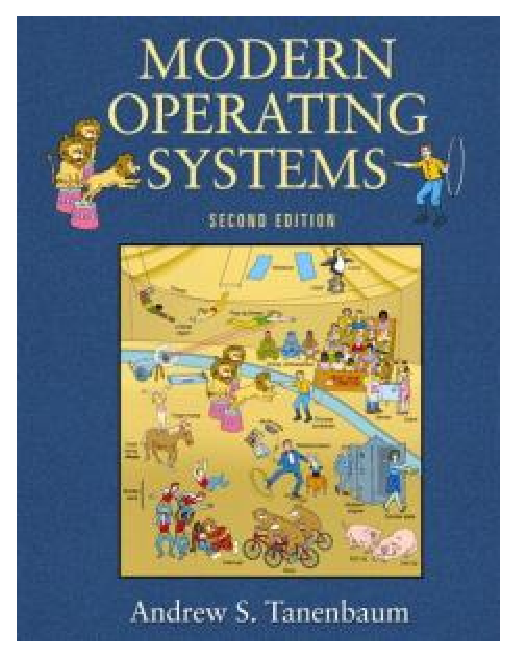
\includegraphics[height=3.5cm]{pics/TanenbaumMOS}
\hspace{2mm}

\includegraphics[height=3.5cm]{pics/TanenbaumDOS}
\end{flushright}
\end{minipage}


\subsection*{Ajánlott irodalom a gyakorlathoz}
\begin{itemize}
\item Rodek Lajos diasorozata a gyakorlathoz (a honlapomról elérhető)
\item Bevezetés a BASH programozásba\\ \url{http://tldp.fsf.hu/HOWTO/Bash-Prog-Intro-HOWTO-hu/Bash-Prog-Intro-HOWTO-hu.html}
\item \textsc{Büki András:} \textit{Héjprogramozás}\\ \url{http://www.kiskapu.hu/index.php?BODY=BookInfo&OP=details&ID=33247}
\item A GAWK felhasználói kézikönyv (letölthető!)\\ \url{http://hexahedron.hu/personal/peteri/gawk/index.html}
\end{itemize}

\subsection*{Linkek}
\subsubsection*{Linux}
\begin{itemize}
\item Általános: \url{http://www.linux.org/}, \url{http://www.linux.hu/}
\item Dokumentációk magyarul: \url{http://www.szabilinux.hu/index.html}
\item Fórum: \url{http://www.linuxempire.hu/}
\item Linux egyszerűen: \url{http://linuxegyszeruen.homelinux.org/}
\item Debian:
			\url{http://www.debian.org/}, 
			\url{http://www.aboutdebian.com/}
\item Ubuntu: 
			\url{http://www.ubuntu.com/},
			\url{http://ubuntu.hu/}%,
%			\url{http://women.ubuntu.hu/}
\end{itemize}

\subsubsection*{Gyakorlatvezetők weboldalai}
\begin{itemize}
\item \url{http://www.stud.u-szeged.hu/Najzer.Helga} (Najzer Helga)
\item \url{http://novakgabor.info} (Novák Gábor)
\item \url{http://www.stud.u-szeged.hu/Santa.Zsolt.1} (Sánta Zsolt)
\end{itemize}

\subsubsection*{Egyetem}
\begin{itemize}
\item \href{http://www.u-szeged.hu/}{Szegedi Tudományegyetem honlapja}
\item \href{https://www.etr.u-szeged.hu/}{SZTE Egységes Tanulmányi Rendszer}
\item \href{http://www.inf.u-szeged.hu}{SZTE Informatika Tanszékcsoport}
\end{itemize}


%	\vfill\pagebreak

\section{Alapok}

\pagenumbering{arabic}
	\subsection{Terminálok}

\begin{center}
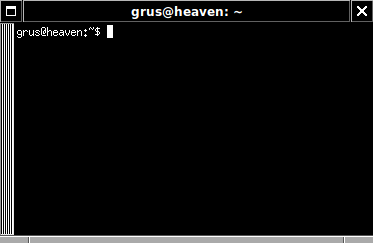
\includegraphics[width=0.6\textwidth]{pics/xterm}

xterm\bigskip


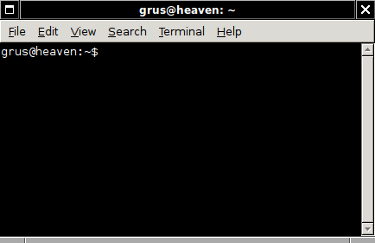
\includegraphics[width=0.6\textwidth]{pics/gnome-terminal}

gnome-terminal\bigskip

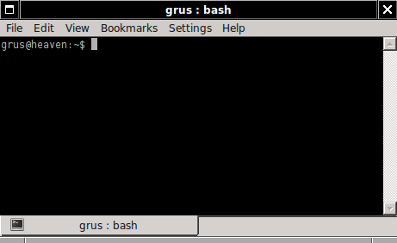
\includegraphics[width=0.6\textwidth]{pics/konsole}

konsole
\end{center}
\pagebreak

\subsection{Alapparancsok}
\subsubsection*{Segítség -- \texttt{man,info}}
\Ovalbox{\large \verb.man. - formázza és kiírja az on-line kézikönyvlapokat }
\medskip

Példa: \texttt{man man} (kilépés: \texttt{q}), man ls (lásd alább)

\begin{lstlisting}
NAME
       ls - list directory contents
SYNOPSIS
       ls [OPTION]... [FILE]...
DESCRIPTION
\end{lstlisting}

%       List information about the FILEs (the current directory by default).  Sort entries alphabetically if none of -cftuvSUX nor --sort is specified.

\subsubsection*{Aktuális könyvtár -- \texttt{pwd, cd}}

\begin{itemize}
\item[]\Ovalbox{\large \verb.pwd. - kiírja az aktuális (munka-) könyvtárat}
	\hfill\texttt{pwd}
	
\item[]\Ovalbox{\large \verb.cd. - az aktuális könyvtár megváltoztatása}
	\hfill\texttt{cd könyvtár}
\end{itemize}

\begin{lstlisting}
joe@localhost:~$ pwd
/home/joe
joe@localhost:~$ cd Documents/
joe@localhost:~/Documents$ pwd
/home/joe/Documents
\end{lstlisting}




\subsubsection*{Létrehozás -- \texttt{mkdir, touch}}
\begin{itemize}
\item[] \Ovalbox{\large \verb.mkdir. - könyvtár létrehozása }
	\hfill \texttt{ mkdir [  kapcsolók  ]   könyvtár}

A \verb.mkdir. Létrehozza a megadott nevű könyvtár(ak)at. 

\medskip

	\textit{Kapcsolók}
	\begin{description}
	\item[-p] Létrehozza a szülőkönyvtárakat is
	 \item[-m jog] A megadott hozzáférési joggal hozza létre a könyvtárakat (később majd ezekről lesz szó)
	\end{description}

\item[] \Ovalbox{\large \verb.touch. - fájl időbélyegének megváltoztatása }
	\hfill\texttt{touch  [-acm][-r   reffájl  |-t   idő  ]   fájl}
	
A \verb.touch. megváltoztatja a megadott fájl(ok) utolsó elérésének és/vagy utolsó módosításának idejét. Ha a fájl nem létezik, a \verb.touch. létrehozza.
\medskip

	\textit{Kapcsolók}
	\begin{description}
	\item[-c, --no-create] Nem hozza létre a fájlokat, ha nem léteznek
	\item[-d, --date= idő] Az idő argumentumot használja az aktuális idő helyett. Ebben lehetnek hónapnevek, időzóna, \texttt{am} vagy \texttt{pm}, stb. 
	\end{description}

\end{itemize}

\begin{lstlisting}
joe@localhost:~/Documents$ ls -lh
total 4.0K
-rw-r--r-- 1 joe joe 827  2011-01-24 01:06 Vicc.txt
joe@localhost:~/Documents$ touch Vicc.txt 
joe@localhost:~/Documents$ ls -lh
total 4.0K
-rw-r--r-- 1 joe joe 827  2011-pics-05 11:44 Vicc.txt
joe@localhost:~/Documents$ mkdir -p newdir/01/pics
joe@localhost:~/Documents$ ls newdir
01
joe@localhost:~/Documents$ ls newdir/01/
pics
\end{lstlisting}




\subsubsection*{Másolás, áthelyezés -- \texttt{cp, mv}}
\begin{itemize}
\item[] \Ovalbox{\large \verb.cp. - fileok másolása} 
	\hfill \texttt{cp [kapcsolók] forrás cél}
\medskip

	\textit{Kapcsolók}
	\begin{description}
	\item[-f] (force) A létező célfájlok törlése
	\item[-i] (interactive) A felhasználó megkérdezése arról, hogy felülírhatók-e a létező célfájlok
	\item[-r,-R] (recursive) A könyvtárak rekurzív másolása, A nem-könytár fájlokat reguláris fájlként másolja 
	\item[-u] (update) Nem másolja azokat a nem-könyvtár fájlokat, amelyeknek azonos vagy újabb módosítási idővel rendelkező célfájlja létezik
	\end{description}


\item[] \Ovalbox{\large \verb.mv. - fileok mozgatása/áthelyezése}
	\hfill\texttt{mv [kapcsolók] forrás cél}
	\medskip
	
	\textit{Kapcsolók}
	\begin{description}
	\item[-f] A létező célfájlok törlése kérdezés nélkül
	\item[-i] A felhasználó megkérdezése arról, hogy felülírhatók-e a létező célfájlok
	\item[-u] Nem mozgatja azokat a nem-könyvtár fájlokat, amelyeknek azonos vagy újabb módosítási idővel rendelkező célfájlja létezik
	\end{description}
\end{itemize}



\subsubsection*{Törlés -- \texttt{rm,rmdir}}
\begin{itemize}
\item[] \Ovalbox{\large rm - állományok eltávolítása}
	\hfill\texttt{rm [ kapcsolók ] fájl(ok)}
	\medskip
	
	\textit{Kapcsolók}
	\begin{description}
	\item[-f] Figyelmen kívül hagyja a nem létező állományokat és nem kérdezi meg a felhasználót
	\item[-i]  Minden fájl eltávolítása előtt megkérdezi a felhasználót, hogy törölheti-e az adott állományt
	\item[-r, -R] A könyvtárak tartalmát rekurzívan törli
	\item[-v] (verbose) Kiírja minden fájl nevét mielőtt törölné
	\end{description}
	
\item[] \Ovalbox{\large rmdir - törli az üres könyvtárakat}
	\hfill\texttt{rmdir [ kapcsolók ] könyvtár(ak)}
	\medskip
	
	\textit{Kapcsolók}
	\begin{description}
	\item[-p] a szülőkönyvtárakat is törli
	%\item[-v] 
	\end{description}
\end{itemize}


\subsubsection*{Kiiratás -- \texttt{cat,less,more}}
\begin{itemize}
\item[] \Ovalbox{\large \verb.cat. - fájlokat fűz össze és kiírja a szabványos kimenetre }
\\
\hspace*{1em}\hfill\texttt{cat [ kapcsolók ] [ file(ok) ]}
	
	
	A cat program minden argumentumként megadott fájlt a szabványos kimenetre ír. Amennyiben nincs fájlnév megadva, vagy a megadott fájlnév a \verb.'-'.-jel, a szabványos bemenetet olvassa. 

\item[] \Ovalbox{\large \verb.more.}
	\hfill\texttt{more [ kapcsolók ] [ -méret ] [ +/ minta ] [ +kezdősor ] [  file(ok) ]}
\item[] \Ovalbox{\large \verb.less.}
	\hfill\texttt{}
	
	A more egy egyszerű szűrőprogram, egy adott szövegből csak egy képernyőnyit mutat. A less egy sok új és hasznos szolgáltatást nyújtó more-emuláció. 
\end{itemize}

	\begin{lstlisting}
	cat fajl.txt
	less fajl.txt
	more fajl.txt
	cat fajl1.txt fajl2.txt
	\end{lstlisting}


\subsubsection*{Filetípus}
\Ovalbox{\large \large\verb.file. - filetípus meghatározása}
	\hfill\texttt{file [ kapcsolók ] [ -f lista ] [ -m bűvösfájl ]  fájl(ok)}\medskip

A file parancs teszteli minden argumentumát és megpróbálja kategorizálni ezeket. %Három teszt sorozatot hajt végre, a következő sorrendben: fájlrendszer tesztek, bűvösszám (magic number) tesztek, és nyelv tesztek. Az első sikeres teszt eredménye határozza meg a program kimenetét.
\bigskip

\begin{lstlisting}
joe@localhost:~/Documents$ ls
Kep001.jpg  Logo.png  newdir  SzegedTreebank.pdf  Vicc.txt
joe@localhost:~/Documents$ file *
Kep001.jpg:         JPEG image data, JFIF standard 1.01, comment: "GIMP"
Logo.png:           PNG image, 180 x 120, 8-bit/color RGBA, non-interlaced
newdir:             directory
SzegedTreebank.pdf: PDF document, version 1.4
Vicc.txt:           UTF-8 Unicode text, with very long lines
\end{lstlisting}


\subsubsection*{Fileok listázása}
\Ovalbox{\large \large \verb.ls. - könytár tartalmának listázása}
	\hfill\texttt{ls [ kapcsoló(k) ] [ file(ok) ]}
	\medskip

	\textit{Kapcsolók}
	\begin{description}
	\item[-1] (egy)  minden sorban csak egy név látszik (egyoszlopos mód)
	\item[-l]  (kis L) hosszú avagy bővített lista
	\item[-a]  a listában a rejtett állományok/könyvtárak is megjelennek 
	
		\emph{Megjegyzés:} rejtett állományok a \verb@.@ (pont)-tal kezdődőek
	\item[-R]  a megadott könyvtár(ak) minden alkönyvtárának és azok teljes tartalmának listázása (rekurzív listázás)
%	\item[-r]  csökkenő sorrend
	\item[-h] olvashatóbb formában írja ki a fileok méreteit 
	\end{description}

%\subsection{Szövegszerkesztők}
%\begin{center}
%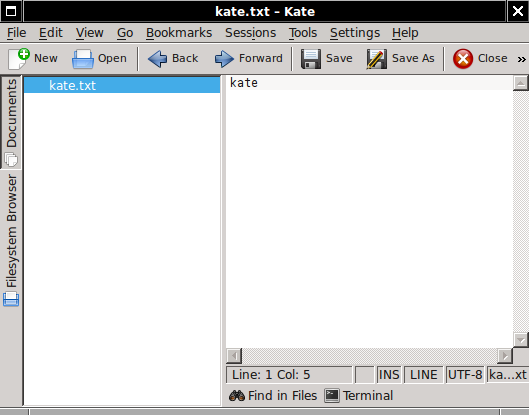
\includegraphics[height=170px]{pics/kate}\hfill
%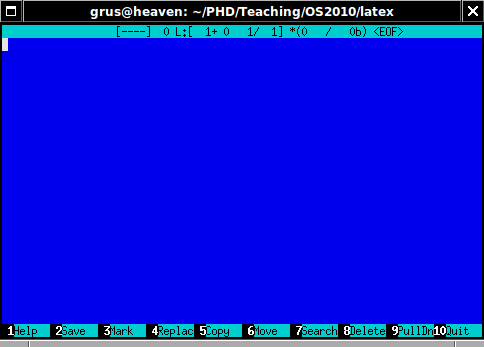
\includegraphics[height=170px]{pics/mcedit}
%\\
%kate\hfill mcedit
%\medskip
%
%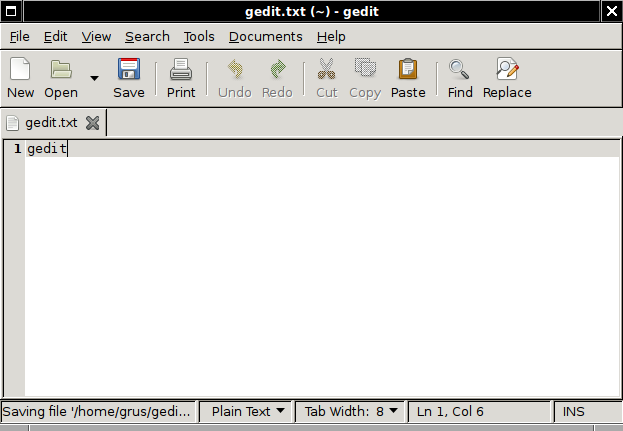
\includegraphics[height=170px]{pics/gedit}\hfill
%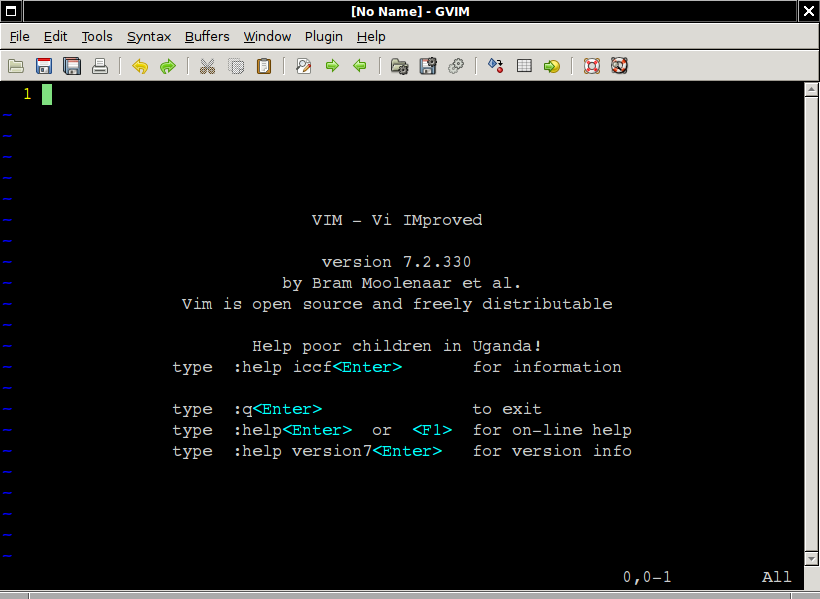
\includegraphics[height=170px]{pics/gvim}
%\\
%gedit \hfill gvim
%\end{center}

\subsection{basename, dirname}
\Ovalbox{\large \large\verb.basename útvonal.}

\begin{quotation}
A könyvtárak neveit eltávolítja a megadott útvonalból (csak az utolsó / utáni állománynév marad meg), majd kiírja az eredményt. Nem ellenőrzi az útvonal valódiságát!
\end{quotation}

\noindent\Ovalbox{\large \large\verb.dirname útvonal.}
\begin{quotation}
Az állomány nevét eltávolítja a megadott útvonalból (csak az utolsó \verb./. előtt álló könyvtárak listája marad meg), majd kiírja az eredményt. Ha az útvonal nem tartalmaz \verb./. jelet, az eredmény a \verb@.@ lesz. Nem ellenőrzi az útvonal valódiságát!
\end{quotation}

%Például:
\begin{lstlisting}
joe@localhost:~$ dirname /usr/bin/nemletezofilenev
/usr/bin
joe@localhost:~$ basename /usr/bin/nemletezofilenev
nemletezofilenev
\end{lstlisting}


%\clearpage

\subsection{Mintaillesztés}
Hasonló felépítésű állomány- vagy könyvtárnevek listájának megadására használhatunk ún. \textit{állománynév mintákat} (filename pattern). Ezek a közönséges karakterek mellett helyettesítő, mintaillesztő avagy Joker-karaktereket is tartalmaznak.
\medskip

\textit{Eredmény:} a mintának megfelelő (mintára illeszkedő) létező nevek szóközökkel tagolt rendezett listája

\subsubsection*{Mintaillesztő karakterek}
\begin{description}
\item{\tt *} tetszőleges karakterekből álló, tetszőlegesen hosszú szó (üres szó is)
\item{\tt ?} egyetlen tetszőleges karakter
\item{\tt[HALMAZ]} A halmaz bármely karakterének egy példánya. A halmazt a karakterek egymás mellé írásával adhatjuk meg.
\item{\tt[ELSŐ-UTOLSÓ]} mint előbb, de itt egy tartományt adunk meg
\item{\tt[\verb.^.HALMAZ]} a halmazban nem szereplő bármely karakter egy példánya
\end{description}

\subsubsection*{Speciális esetek}
Mindig ki kell írni a rejtett állományok/könyvtárak nevének kezdő pont (.) karakterét, ill. könyvtárak esetén a könyvtárnév után a / jelet.

A pont karakter egyéb esetekben nem számít speciálisnak. Néhány program azonban az állománynevekben az utolsó pont utáni részt, az ún. \emph{kiterjesztést} (filename extension) különlegesen kezeli. Ezt általában az állomány tartalma típusának jelzésére használják (pl. kép, video, hang).\bigskip

\noindent\textit{Példák}
\begin{description}
\item{\bf *} az összes nem rejtett állomány és alkönyvtár
\item{\bf */} az összes nem rejtett alkönyvtár
\item{\bf */*} az összes nem rejtett alkönyvtár teljes tartalma
\item{\bf .*} az összes rejtett állomány és alkönyvtár
\item{\bf .*/} az összes rejtett alkönyvtár
\item{\bf *.jpg} a .jpg kiterjesztésű állományok (JPEG formátumú képek)
\item{\bf *.*} az összes nem rejtett állomány és alkönyvtár, amelynek neve tartalmaz legalább egy pontot
\end{description}


%\textit{Példák}
\begin{lstlisting}
joe@localhost:~/dir$ ls -a
.                 ebay_fanshop.png  hello.sh  pepita_sakk.png  ubigraph1.png
..                file.txt          Judy.png  .rejtett1        ubigraph2.png
BatteryLinux.png  final.png         Logo.png  .rejtett
joe@localhost:~/dir$ ls *
BatteryLinux.png  file.txt   hello.sh  Logo.png         ubigraph1.png
ebay_fanshop.png  final.png  Judy.png  pepita_sakk.png  ubigraph2.png
joe@localhost:~/dir$ ls ?ello.sh
hello.sh
joe@localhost:~/dir$ ls ubigraph[12].png
ubigraph1.png  ubigraph2.png
joe@localhost:~/dir$ ls ubigraph[0-9].png
ubigraph1.png  ubigraph2.png
joe@localhost:~/dir$ ls .*
.rejtett1  .rejtett2
joe@localhost:~/dir$ ls *.png
BatteryLinux.png  final.png  Logo.png         ubigraph1.png
ebay_fanshop.png  Judy.png   pepita_sakk.png  ubigraph2.png
\end{lstlisting}


\subsection{Keresés}
\Ovalbox{\large \large\verb.locate. -- mintához illeszkedő fájlokat nyomtat a fájlnév adatbázis(ok)ból}\medskip

\hfill\texttt{locate [ -d   elérési út  ] [ --database=  elérési út  ] [ --version ] [ --help ] minta...}
\medskip

\begin{quotation}
\small
A locate parancs végignézi a megadott fájlnév-adatbázis(oka)t és kinyomtatja azokat a fájl\-ne\-ve\-ket, melyek illeszkednek a mintá(k)ra. A minták tartalmazhatnak shell-stílusú speciális karaktereket is (metakarakterek). Ezek a: '*', '?', és '[]'. A metakarakterek nem kezelik a '/' vagy '.' karaktereket speciálisan, emiatt például a 'foo*bar' minta illeszkedik a 'foo3/bar' karaktersort tartalmazó fájlnévre, hasonlóan a '*duck*' minta is illeszkedik a 'lake/.ducky' karaktersort tartalmazó fájlnevekre. A metakaraktereket tartalmazó mintákat idézőjelek közé kell tenni jelezve, hogy azok nem a parancsértelmezőnek (shell) szólnak. 
\end{quotation}

\noindent\Ovalbox{\large \large\verb.find. -- fájlokat keres egy könyvtárstruktúrában}
	\medskip

	\hfill\texttt{find [útvonal...] [kifejezés] }\medskip


%\begin{quotation}
A find parancs rengeteg kapcsolóval rendelkezik, emellett operátorokat is használhatunk vele, részletesebben lásd \texttt{man find}.
%\end{quotation}
\bigskip

	Álljon itt néhány példa a teljesség igénye  nélkül\footnote{A legtöbb példa a \url{http://linuxbox.hu/find} oldalról származik}.
	Keressünk\dots
	\begin{itemize} 
	\item  \texttt{.jpg} fájlokat az aktuális könyvtárakban így: \verb@find . -name *.jpg@

	\item 20 évnél idősebb állományokat keresünk az aktuális könyvtárban így: \verb@find ./ -mtime +7300@
	\item az utolsó 3 napban módosított állományokat így:	\verb@find . -mtime -3.@

	\item az utolsó 3 napban módosított txt állományokat így: \verb@find . -name '*.txt' -mtime -3@
	
	\item 10000 kbytenál nagyobb állományokat így: \verb@find . -size +10000k@


	\item rc.conf nevű állomány keresése az aktuális könyvtárban
	\begin{lstlisting}
	find . -name "rc.conf" -print
	\end{lstlisting}

	\item ha megtalálta a find az rc.conf nevű állományt akkor azon végre hajtja a chmod utasítást
	\begin{lstlisting}
	find . -name "rc.conf" -exec chmod o+r '{}' \;
	\end{lstlisting}

	\item komplex keresés ami kihagyja az eredményből a *.v vagy .*.v nevű állományokat. Egy kis extra ma\-gya\-rá\-zat: -not negálást jelent, -o a logikai OR műveletet, $\backslash($ a logikai művelet kezdetét jelöli, $\backslash)$ pedig a végét. Egyébként a kihagyott állományok egy verzió kezelő állományai...
	\begin{verbatim}
	find /usr/src -not \( -name "*,v" -o -name ".*,v" \) '{}' \; -print
	\end{verbatim}

	\item keresés a linuxbox szóra a *.html nevű állományokban, állomány név kiiratás találat esetén.
	\begin{lstlisting}
	find . -name "*.html" -exec grep "linuxbox" '{}' \; -print
	\end{lstlisting}

	\item Keresés az aktuális könyvtárból indulva kis és nagybetű nem figyelembe vételével és kihagyni a .svn nevű könyvtárak tartalmát:
	\begin{lstlisting}
	find . -iname "*old*" -a -not -path "*.svn*" -print
	\end{lstlisting}

	Itt igazából az \texttt{-and -or -not} keresési feltételek közti logikai művelet megadás lehetősége a lényeg!

	\end{itemize}

\subsection{Állománynév-kiegészítés}
A hosszabb nevek begépelését könnyíti meg az \emph{állománynév-kiegészítés} (filename completion). A név első pár betűjének beírása után üssük le a \Tab\footnote{Tab} billentyűt. Ha csak egy állomány neve kezdődik így, akkor a név kiegészül. Különben még egyszer üssük le a \Tab-ot, hogy egy listát kapjunk a szóba jöhető nevekről. Ezután folytassuk a gépelést a kívánt karakterrel. Ez a szolgáltatás könyvtár- és programneveknél is működik.




%	\vfill\pagebreak

\section{Jogosultságok, csatornák, szöveges fájlok, felhasználók}
	
\subsection{Jogosultságok}

\begin{itemize}
\item minden állománynak van tulajdonosa és csoportja 
\item mindezekhez tartozik 
	\begin{description}
	\item[r] olvasási jog

\begin{quotation}
\small		
	Ha a tulajdonosnak az olvasási jogát jelző kapcsoló be van kapcsolva, akkor az adott állományban található adatokat a tulajdonos megnézheti, olvashatja, kinyomtathatja, lemásolhatja, egy szóval az adatokhoz hozzáférhet. Ha e kapcsoló ki van kapcsolva, akkor az állomány nevét látja ugyan a tulajdonos, de a tartalmához nem férhet hozzá.


A \textit{könyvtáron értelmezett olvasási jog} a benne található állományok nevének kilistázását jelenti. Ha ezzel a joggal rendelkezik valaki akkor listázhatja az állományokat az adott könyvtárban, ha nem, akkor ezt nem teheti meg. Ötletes módon, az állományokat esetleg létrehozhatja, és akár módosíthatja is, attól függetlenül, hogy róluk listát nem kaphat.
\end{quotation}

	\item[w] írási jog

\begin{quotation}
\small	
	A tulajdonos írási jog kapcsolója megmutatja, hogy a számára engedélyezett-e az adatok írása, vagyis módosítása. Ha ez be van kapcsolva, akkor a tulajdonos módosíthatja, bővítheti és törölheti az adott állományban található adatokat, sőt törölheti akár az egész állományt. Ha e kapcsoló ki van kapcsolva, akkor a tulajdonos nem módosíthatja az adatokat, még az állomány végére sem fűzhet újabb információkat.
	
A \textit{könyvtáron értelmezett írási jog} újabb fájlok létrehozására és törlésére ad lehetőséget. Ha írási joggal nem rendelkezik valaki az adott könyvtárban, esetleg még írhat a benne levő állományokba vagy azokból adatokat törölhet. Egész állományokat nem hozhat létre és egész állományokat viszont nem törölhet. Amennyiben a könyvtárból az ott található állományokat nem tudja a felhasználó kitörölni, a könyvtárat magát sem tudja törölni, hiszen csak üres könyvtárakat lehet kitörölni. Ha a könyvtár már üres, a felhasználónak nincs szüksége írási jogra a könyvtárra nézve ahhoz, hogy azt kitörölhesse.
\end{quotation}


	\item[x] futtatási jog
	
\begin{quotation}
\small	
	A tulajdonos futtatási jogát jelzőkapcsoló azt mutatja meg, hogy a tulajdonos elindíthatja-e az adott állományt. Ennek a lehetőségnek csak programok esetében van értelme. %, adatokat tartalmazó állomány esetében e kapcsoló ki van kapcsolva.
	
A \textit{könyvtáron értelmezett futtatási jog} a könyvtár megnyitását jelenti, vagyis azt a képességet, hogy a könyvtárba belépjünk.


\end{quotation}
	\end{description}

\item fájl(ok) futtatásához és mappa megnyitáshoz is \texttt{rx} (olvasási és futtatási) jog szükséges
\end{itemize}
\bigskip

\noindent{\large\Ovalbox{\verb.chmod. - fájlok elérési jogainak megváltoztatása }
	\hfill \texttt{chmod +|-<mód> <fájlnév>}}
	\medskip
	
Egy fájl tulajdonosi (hozzáférési) jogait csak a fájl tulajdonosa, vagy a rendszergazda tudja megváltoztatni. A továbbiakban tegyük fel, hogy a \texttt{pelda.txt} file tulajdonosa  mi vagyunk.
\begin{description}
\item[+/-:] ezzel jelezzük, hogy adunk vagy elveszünk jogot.
\item[mód]: két dolgot kell ezesetben meghatároznunk\medskip

	\textit{kinek adunk}
	\begin{description}
	\item[u] pl. \texttt{chmod u+w pelda.txt} - saját magunknak írási jog
	\item[g] pl. \texttt{chmod g+r pelda.txt} - csoportnak olvasási jog
	\item[o] pl. \texttt{chmod o+x pelda.txt} - másoknak futtatási jog
	\item[a] (all -- mindenki)  \texttt{chmod a+rwx pelda.txt} - mindenkinek megadjuk az olvasási, írási és futtatási jogot
	\end{description}
	
	\textit{\dots és milyen jogot}
	\begin{description}
	\item[r,w,x] (lásd feljebb)
	\end{description}
	
	Lehet kombinálni is a fentieket, pl. \texttt{\$chmod ug+w pelda.txt}
\bigskip
	
Ha a csoportot -- akire az adott jog vonatkozik -- nem adjuk meg, akkor az mindhárom csoportra vonatkozik:
\begin{lstlisting}
joe@localhost:~$ ls -l fajl.txt 
-rw-r--r-- 1 joe joe 178 2011-02-11 18:45 fajl.txt
joe@localhost:~$ chmod +x fajl.txt
joe@localhost:~$ ls -l fajl.txt 
-rwxr-xr-x 1 joe joe 178 2011-02-11 18:45 fajl.txt	
\end{lstlisting}


Ha nem a \verb.+. vagy \verb.-. jeleket használjuk, hanem az \verb.=. jelet, akkor azok a jogok kapcsolódnak be, amelyeket felsorolunk, a többi pedig visszavonásra kerül:

\begin{lstlisting}
joe@localhost:~$ ls -l fajl.txt 
-rwxr--r-- 1 joe joe 178 2011-02-11 18:45 fajl.txt
joe@localhost:~$ chmod u=rw fajl.txt 
joe@localhost:~$ ls -l fajl.txt 
-rw-r--r-- 1 joe joe 178 2011-02-11 18:45 fajl.txt
\end{lstlisting}



\end{description}

A jogosultságok  megváltoztatásakor nem csak a fenti mód használható, hanem számszerű formátumban  is megadhatjuk a jogokat. 

A jobb oldalon látható táblázat adja meg melyik joghoz milyen szám tartozik. Ha több jogot szeretnénk alkalmazni, akkor össze kell adnunk az értékeket, például az 5 az olvasási és futtatási jogot jelenti, a 6 az olvasásit és írásit. 
\begin{center}
\small
\begin{tabular}{lccc}
\toprule
	Jogok 	&\bf u 		&\bf g 		&\bf o\\
	 	&tulajdonos 	&csoport	&mindenki más\\
\midrule
\bf Olvasás 	&r 		&r		&r\\
\bf Írás	&w 		&w 		&w\\
\bf Futtatás 	&x 		&x 		&x\\
\bottomrule

\end{tabular}
\hfill
\begin{tabular}{lccc}
\toprule
	Jogok 	&\bf u 		&\bf g 		&\bf o\\
	 	&tulajdonos 	&csoport	&mindenki más\\
\midrule
\bf Olvasás 	&4 		&4 		&4\\
\bf Írás	&2 		&2 		&2\\
\bf Futtatás 	&1 		&1 		&1\\
\bottomrule
\end{tabular}
\end{center}

\bigskip

\textit{Példák}
Az alábbi táblázatban az egymás mellett levő parancsok ekvivalensek.
\begin{center}
\begin{tabular}{l|l}
\toprule
chmod u=rw,g=r,o=r fajl.txt	& chmod 644 fajl.txt\\
chmod ugo=rw fajl.txt		& chmod 666 fajl.txt\\
chmod a=rwx fajl.txt		& chmod 777 fajl.txt\\
chmod ugo-rwx fajl.txt	 	& chmod 000 fajl.txt\\
\bottomrule
\end{tabular}
\end{center}
\bigskip

{
\noindent\Ovalbox{\large\verb.chown. - fájlok felhasználói és csoport tulajdonosának megváltoztatása}
\medskip

       \hfill \texttt{chown [ kapcsolók ] [ tulajdonos ][:[ csoport ]] file(ok)}
       }\bigskip
       
       
A \verb.chown. (change owner, tulajdonosváltás) parancs segítségével megváltoztathatjuk az állomány tulajdonosát és csoporttulajdonosát. Alapesetben -- ha csak a tulajdonost változtatjuk -- a parancsnak a tulajdonos nevét és az állománynevet kell megadnunk:

\begin{lstlisting}
joe@localhost:~$ ls -l fajl.txt 
-rw-r--r-- 1 joe    joe 178 2011-02-11 18:45 fajl.txt
joe@localhost:~$ chown andrea fajl.txt 
joe@localhost:~$ ls -l fajl.txt 
-rw-r--r-- 1 andrea joe 178 2011-02-11 18:45 fajl.txt
\end{lstlisting}

Ha a csoporttulajdonost is meg akarjuk változtatni, akkor a tulajdonos neve után kettősponttal elválasztva kell az új csoportot megadnunk:

\begin{lstlisting}
joe@localhost:~$ chown joe:csoportnev fajl.txt
joe@localhost:~$ ls -l fajl.txt 
-rw-r--r-- 1 joe csoportnev 178 2011-02-11 18:45 fajl.txt
\end{lstlisting}

\medskip
\textit{Kapcsolók}
\begin{description}
\item[-R] rekurzívan változtatja meg a (paraméterként megadott) könyvtár és annak tartalmának tulajdonosát
\end{description}
\bigskip

\noindent\Ovalbox{\large\verb.chgrp. - fájlok tulajdonosi csoportjának megváltoztatása }\bigskip

A \verb.chgrp. (change group ownership, csoporttulajdonos megváltoztatása) paranccsal megváltoztathatjuk az állományok és könyvtárak csoport tulajdonosát. Erre alkalmas a \verb.chown. parancs is, ha azonban csak a csoporttulajdonost kívánjuk megváltoztatni (a tulajdonost nem) akkor erre a feladatra a \verb.chgrp. használható.


\begin{lstlisting}
joe@localhost:~$ chgrp csoportnev fajl.txt
joe@localhost:~$ ls -l fajl.txt 
-rw-r--r-- 1 joe csoportnev 178 2011-02-11 18:45 fajl.txt
\end{lstlisting}

%\end{itemize}



\subsection{Standard csatornák és az átirányítás}
A Unixban 3 standard be- és kimeneti csatorna van definiálva:
\begin{description}
\item[standard bemenet] (stdin, 0)
\item[standard kimenet] (stdout, 1)
\item[standard hibacsatorna] (stderr, 2)
\end{description}
 
 Alapértelmezésben a standard bemenet a billentyűzet, a kimenet és a hibacsatorna pedig a képernyő (többnyire a terminál). Az átiranyítás lényege, hogy a programot utasíthassunk arra, hogy a bemenetet ne a billentyűzetről várja, illetve eredményeit ne a képernyőre (terminálba) írja ki. 
 
 \begin{description}
 \item[bemenet átirányítása] \verb.<. \ például: \texttt{cat < fajl.txt}
 \item[kimenet átirányítása] \verb.>. \ például: \texttt{cat fajl.txt > file2.txt} 
 
 	A \texttt{fajl.txt} tartalmát a \texttt{file2.txt}be irányítjuk.\\
 	A fenti parancs tulajdonképpen egyenértékű a \texttt{cp fajl.txt file2.txt} paranccsal
 \item[hibacsatorna átirányítása] \verb.2>. \ például: \texttt{du -h / 2>/dev/null}
 \medskip
 
 \textit{,,Speciális'' átirányítások: }
 \item[2>\&1:] a stderr-t ugyanoda irányítja, ahová a stdout irányítva lett
\item[1>\&2:] a stdout-ot ugyanoda irányítja, ahová a stderr irányítva lett

 \end{description}
	
\noindent{\color{red}\textbf{Megjegyzés:}} a \verb.>. átirányítás felülír. Ezért ha egy létező file végéhez szeretnénk hozzáfűzni átirányítás során, akkor használjuk a \verb.>>. formában megadott \textit{adaptív} átirányítást. 


\subsection{\texttt{|}, a csővezeték}
Ha egy parancs kimenetét szeretnénk  egy másik parancs bemenetére irányítani, arra az  ún. csővezeték (pipe) alkalmas, melyet a  \verb.|. karakter reprezentál. \bigskip

\emph{Példák}

\begin{itemize}
\item \verb.ls | wc -w. \hfill Hány állomány van az aktuális könyvtárban? 
\item \verb.ls | sort | less. \hfill Lapozható, sorbarendezett állománylista
\end{itemize}


\subsection{tee}
\hfill\texttt{tee [-ai]  [--ignore-interrupts] [ fájl... ]}
\begin{quotation}
A \verb.tee. parancs a standard bemenetén kapott adatokat a standard kimenetre és valamennyi argumentumként kapott fájlba másolja. Ez akkor hasznos, ha az adatokat nemcsak a csővezetéken szeretnénk továbbítani, hanem szükségünk van egy másolatra is.
\end{quotation}
\bigskip


\textit{Kapcsolók}
\begin{description}
\item[-a, -{}-append] A standard bemenet tartalmát a célfájlok végéhez fűzi, és nem írja felül azokat.
\item[-i, -{}-ignore-interrupts] Figyelmen kívül hagyja a megszakításra vonatkozó jelzéseket.
\item[-{}-help] Használati útmutatót ír a standard kimenetre, majd sikeres visszatérési értékkel kilép.
\item[-{}-version] A program verziójáról ír ki információt a standard kimenetre, majd sikeres visszatérési értékkel kilép.
\end{description}

\begin{center}
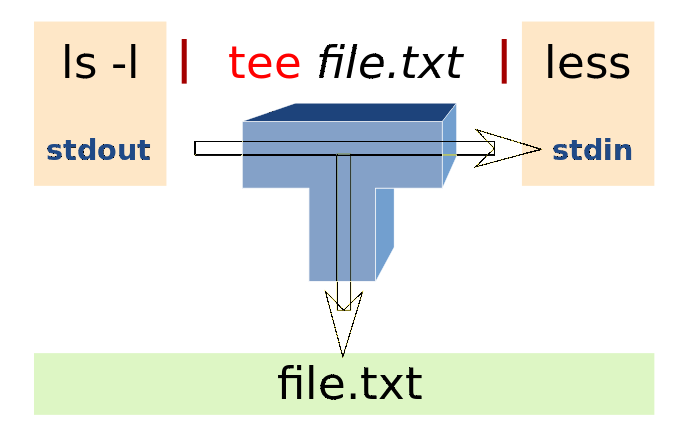
\includegraphics[width=0.5\textwidth]{pics/Tee2}\\
\footnotesize
Kép forrása: \url{http://hu.wikipedia.org/wiki/Tee_\%28parancs\%29}
\end{center}

\subsubsection*{Példa (1)}
Nézzünk a csővezeték és a \verb.tee. együttes használatára egy példát! Tegyük fel, hogy van egy fájlunk, melynek minden sorában egy név áll. A \verb.sort. parancs segítségével a \verb@nevsor_kevert.txt@ tartalmát sorbarendezzük. A sorbarendezés eredménye a \verb.tee. parancs hatására megjelenik a standard kimeneten (terminál) illetve a \verb@nevsor.txt@ fájlban is.

\begin{lstlisting}
joe@localhost:~$ cat nevsor_kevert.txt 
Kocsis Attila
Dobi Imre
Toth Zoltan
Kormanyos Jozsef Sandor
Lok Arpad
Botas Zoltan
Baranyi Peter
Buza Endre Csongor
joe@localhost:~$ cat nevsor_kevert.txt |sort|tee nevsor.txt
Baranyi Peter
Botas Zoltan
Buza Endre Csongor
Dobi Imre
Kocsis Attila
Kormanyos Jozsef Sandor
Lok Arpad
Toth Zoltan
\end{lstlisting}


\subsubsection*{Példa (2)}
%\begin{minipage}{0.7\textwidth}

\begin{lstlisting}
joe@localhost:~/tmp/Documents$ ls
BatteryLinux.png  final.png  Judy.png  pepita_sakk.png  ubigraph2.png
fajl.txt          hello.sh   Logo.png  ubigraph1.png
joe@localhost:~/tmp/Documents$ ls | tee fajl.txt
BatteryLinux.png
fajl.txt
final.png
hello.sh
Judy.png
Logo.png
pepita_sakk.png
ubigraph1.png
ubigraph2.png
joe@localhost:~/tmp/Documents$ cat fajl.txt 
BatteryLinux.png
fajl.txt
final.png
hello.sh
Judy.png
Logo.png
pepita_sakk.png
ubigraph1.png
ubigraph2.png
\end{lstlisting}

%\end{minipage}
%\begin{minipage}{0.25\textwidth}

%\end{minipage}


%\clearpage

\subsection{Szöveg kiírása, szöveges fájlok kezelése}
\Ovalbox{\large \texttt{echo} -- kiír egy szövegsort}
	\begin{quotation}
  Az   \verb.echo.  kiír  minden  megadott  karakteláncot a szabványos kimenetre,
       szóközökkel elválasztva és egy újsor karakterrel a  végén,  hacsak  nem
       volt megadva a \verb.-n. opció.
\bigskip

\emph{Kapcsolók}
\begin{description}

\item[-n]   Nem írja ki a sor végére a soremelést karaktert.


\item[-e]    Engedélyezi  a  következő  speciális  karakterek  értelmezését a
              karakterláncokban:
              \begin{description}
              \item[$\backslash$a]     riadó (csengő)
              \item[$\backslash$b]     egy karakter törlése visszafelé
              \item[$\backslash$c]     nem ír ki újsor karaktert
              \item[$\backslash$f]     lapdobás
              \item[$\backslash$n]     új sor
              \item[$\backslash$r]     kocsi vissza
              \item[$\backslash$t]     vízszintes tab
              \item[$\backslash$v]     függőleges tab
              \item[$\backslash\backslash$]     backslash
              \item[$\backslash$nnn]   a karakter ASCII kódja nnn (oktálisan)
              \end{description}

\item[-E]    backslash ($\backslash$) karakterrel megadott karakterek értelmezésének tiltása (alapértelmezett)
\end{description}

\begin{lstlisting}
joe@localhost:~$ echo "Hi all"
Hi all
joe@localhost:~$ echo 'Hi all!'
Hi all!
\end{lstlisting}

\end{quotation}

\clearpage

\noindent\Ovalbox{\large \texttt{printf} -- formátumozott adatkiírás}

   \begin{quotation}
      A printf kinyomtatja a formátum szöveget, értelmezi a '\%' és '$\backslash$' escape
       szekvenciákat ugyanúgy, mint a C \texttt{printf} függvény.  A formátum  argumentumot használja az összes kapott argumentum formázásához.
       
\begin{lstlisting}
joe@localhost:~$ printf "%s\n" "Hello World"  
Hello World
\end{lstlisting}
       \end{quotation}
\bigskip


\noindent\Ovalbox{\large \texttt{wc} -- fájlokban található bájtok, szavak és sorok számát írja ki}
	


\begin{quotation}
       A \verb.wc. program bájtok, szavak és újsor-jelek számát számolja meg az argumentumként megadott fájlokban.  Ha nem adunk meg fájlnevet,  illetve  a fájlnévként a '-' jelet adjuk meg, akkor a szabványos bemenet olvassa a program.

       Alapértelmezés szerint a \verb@wc@ mindhárom számot kiírja. Az opciókkal lehet megadni,  hogy csak bizonyos számok legyenek kiírva. Az opciók nem semlegesítik egymás hatását, így pl.  \verb@wc --bytes --words@  a  bájtok  és  a szavak számát egyaránt kiírja.  Minden fájlról egysornyi információt ír ki, és az argumentumként megadott fájlok nevét is kijelzi. Több fájlnév  esetén egy összesített sort is megad a lista végén \texttt{total} fájlnéven. A megadott adatok sorrendben a következőek: sorok, szavak, bájtok száma.
\bigskip

\textit{Kapcsolók}
\begin{description}
\item[-c, -{}-bytes, -{}-chars]
              Csak a bájtok számát írja ki.

\item[-l, -{}-lines]
              Csak a sorok számát írja ki.

\item[-w, -{}-words]
              Csak a szavak számát írja ki.

\item[-L, -{}-max-line-length]
              Csak a fájlban  előforduló  leghosszabb  sor  hosszát  írja  ki,
              illetve  ha  egynél  több  fájl volt megadva, akkor kiírja még a
              legnagyobbat az előző értékek közül (nem az összegüket írja ki).
\end{description}

\begin{lstlisting}
 joe@localhost:~$ wc os05.tex
  266  1152 11304 os05.tex
\end{lstlisting}

\end{quotation}
%\clearpage

\noindent\Ovalbox{\large \texttt{grep} -- mintához illeszkedő sorokat nyomtat}\footnote{A \texttt{grep} parancs neve a 
  \texttt{sed} parancs \texttt{/g/re/p} utasításából ered, ahol a \texttt{re} a regular expression rövidítése, A \texttt{grep} 
  ugyanis pontosan azt teszi, amit a \texttt{sed} erre az utasításra}

\begin{quotation}
 A \verb.grep. szétválasztja azokat a sorokat, amelyekben a keresett részlet megtalálható azoktól, melyekben nem. A grep alapesetben csak azokat a sorokat választja ki 
(írja ki), melyekben a keresett mintát megtalálta:
\begin{lstlisting}
joe@localhost:~$ ps -e|grep firefox
 3531 ?        00:11:22 firefox-bin
joe@localhost:~$ ps -e |grep kde
 3342 ?        00:00:00 kdeinit4
 3347 ?        00:00:00 kded4
\end{lstlisting}

A \texttt{-v} (revert, ellentétes) kapcsoló hatására a grep  csak azokat a sorokat tengedi tovább, melyekben a keresett
minta nem található meg. 

\begin{lstlisting}
joe@localhost:~$ who|grep joe
joe     tty7         2011-02-26 19:17 (:0)
joe     pts/0        2011-02-26 19:29 (:0.0)
joe     pts/3        2011-02-26 19:45 (:0.0)
joe     pts/1        2011-02-26 20:42 (:0.0)
joe     pts/2        2011-02-26 20:55 (:0.0)
joe@localhost:~$ who|grep -v pts
joe     tty7         2011-02-26 19:17 (:0)
\end{lstlisting}
A \texttt{-i} (ignore, figyelmen kívűl hagy) kapcsoló hatására a grep nem veszi figyelembe a kis- és nagybetűk közti különbséget.

\end{quotation}

%\clearpage

\noindent\Ovalbox{\large head --  fájlok első részének kiírása}
\begin{quotation}
A  \texttt{head}  a  megadott fájlok  első részét (alapértelmezésben első 10 sorát) írja ki. Ha nincs megadva fájlnév, vagy a fájlnév '-', a bemenetét  a  szabványos  bemenetről  veszi.  Ha  egynél  több fájl adott, a fájl nevét '==>' és '<=='
       jelek közé téve minden fájl első része előtt kiírja.
\bigskip

     A head kétfajta opciómegadást fogad el: az újat,  amikor  a  számok  az
       opciókat  jelző  betűknek  argumentumok  és  a  régit,  amikor a számok
       megelőzik az opciókat jelző betűket.

      \begin{description}
       \item[-c N, -{}-bytes N]
         Az első N bájtot írja ki. N nem-nulla egész,  amit  opcionálisan
              követ a következő karakterek közül egy, kijelölendő az egységet:

	    \begin{description}
	     \item[b] 512 bájt hosszú blokk
             \item[k] 1 kilobájt hosszú blokk
             \item[m] 1 megabájt hosszú blokk
	    \end{description}

      \item[-n N, -{}-lines N]
              Az első N sort írja ki.
      \end{description}
 
     
\end{quotation}

\noindent\Ovalbox{\large  \texttt{tail} -- kiírja a meghatározott fájl utolsó részét}

\begin{quotation}
 A tail parancs a megadott fájl(ok) utolsó sorait (10 sor  az  alapértelmezett) írja ki; a szabványos bemenetről olvas, ha nincs fájl megadva, vagy, ha
       a fájl nevet '-' követi.  Ha több, mint egy fájl van megadva, kiír  egy fejlécet, ami tartalmazza a fájl nevét '==>' és '<==' jelek közé zárva,
       a többi fájl kimenetei előtt.

  Kapcsolóit lásd a \texttt{head} parancsnál.
\end{quotation}

%\clearpage

\noindent\Ovalbox{\large \texttt{uniq} -- egy rendezett fájlból kiszedi a duplikált sorokat}
\begin{quotation}

       A \verb.uniq. kiírja az egyedi sorokat egy rendezett  fájlból,  és eldobja  az  egyezőket  egy  kivételével.  
      Opcionálisan,  mutathatja csak azokat a sorokat is, amelyek pontosan megegyeznek, illetve azokat, amelyek egynél többször fordulnak elő. A \verb.uniq.-nak rendezett bemenetre van  szüksége,  mivel
       csak az egymás után következő sorokat hasonlítja össze.

       Ha a kimenet nem specifikált, a \verb.uniq. a szabványos kimenetre ír. Ha a bemeneti file nincs megadva, 
	a standard input-ot  olvassa.
    \bigskip
    
    \emph{Kapcsolók}
    \begin{description}
     \item[-u, -{}-unique]
              Csak a nem azonos sorokat írja ki.

      \item[-d, -{}-repeated]
              Csak a duplikált sorokat írja ki.
    \end{description}
\end{quotation}


\noindent\Ovalbox{\large \texttt{dos2unix} -- szöveges fájlok átalakítására használható DOS/MAC $\rightarrow$ UNIX}

\begin{quotation}
    \emph{Fontosabb kapcsolók}
	\begin{description}
		\item[-k -\-keepdate] a kimeneti fájl időbélyege egyezni fog a bemenetivel
		\item[-c -\-convmode convmode] az átalakítás módja. Lehet: ASCII, 7bit, ISO, Mac, alapértelmezett az ASCII.
	\end{description}
\end{quotation}


\noindent\Ovalbox{\large \texttt{unix2dos} -- szöveges fájlok átalakítására használható UNIX $\rightarrow$ DOS/MAC}


\begin{quotation}
    \emph{Fontosabb kapcsolók}
	\begin{description}
		\item[-k -\-keepdate] a kimeneti fájl időbélyege egyezni fog a bemenetivel
		\item[-c -\-convmode convmode] az átalakítás módja. Lehet: ASCII, 7bit, ISO, Mac, alapértelmezett az ASCII.
	\end{description}
\end{quotation}


\subsection{Felhasználókkal kapcsolatos parancsok}
\noindent\Ovalbox{\large A \verb.who. parancs kilistázza a képernyőre a számítógépre bejelentkezett felhasználókat.}
%
\begin{quotation}
Amennyiben az opciókon kívül nincs argumentuma, a who program kinyomtatja minden, pillanatnyilag bejelentkezett felhasználóról a következő információkat:
\end{quotation}

\begin{itemize}
\item bejelentkezési név (login name) 
\item terminál vonal (terminal line) 
\item a bejelentkezés ideje (login time) 
\item távoli gépnév vagy X kijelző (remote hostname or X display)
\end{itemize}

\begin{lstlisting}
joe@localhost:~$ who
joe     pts/0        2011-02-19 11:03 (:0.0)
joe     pts/1        2011-02-19 12:03 (:0.0)
joe     pts/2        2011-02-19 12:04 (:0.0)
\end{lstlisting}

%Ha egyetlen argumentumot (amely nem opció) adunk meg a parancssorban, akkor a who program az így megadott fájlt használja a  /etc/utmp    helyett a bejelentkezett   felhasználók azonosítására. Szokás a   /etc/wtmp -t használni itt, hogy az előző bejelentkezéseket vizsgálhassuk. 


\noindent\Ovalbox{\large A \verb.whoami. parancs kiírja a felhasználó nevét.}
%
\begin{quotation}
A \texttt{whoami} program kiírja a bejelentkezett felhasználó nevét.
\end{quotation}
\begin{lstlisting}
joe@localhost:~$ whoami
joe
\end{lstlisting}



\noindent\Ovalbox{\large A \verb.finger. parancs a felhasználói információk megjelenítésére szolgál.}

\hfill\texttt{finger [user]}
\medskip

\textit{Kapcsolók}
\begin{description}
\item[-s] A finger megmutatja a felhasználó belépési nevét, valódi nevét, terminálját és hogy az írható-e (a terminál neve mögött ``* jelenik meg, ha nem írható), mióta nem csinált semmit, mikor lépett be, valamint irodájának helyét és telefonszámát. A belépés idejét hónap, nap, óra, perc formában adja meg, kivéve ha hat hónapnál régebben lépett be; ezesetben az óra és a perc helyett az évet jelzi ki. Az ismeretlen eszközök és a nemlétező belépési valamint nyugalmi időt csillaggal jelzi.

\item[-l] Többsoros megjelenítés, amely magában foglalja az \verb.-s. kapcsoló által mutatott adatokat, valamint a felhasználó home mappáját, otthoni telefonszámát, belépési shelljét, leveleinek állapotát és a home mappájában található \verb@.plan@, \verb@.project@ valamint \verb@.forward@ nevű fájlok tartalmát.
\end{description}

\begin{lstlisting}
joe@localhost:~$ finger
Login     Name            Tty     Idle  Login Time   Office     Office Phone
joe      Joe C.  	 pts/0       4  Feb 19 11:03 (:0.0)
joe      Joe C.  	 pts/1    1:05  Feb 19 12:03 (:0.0)
joe      Joe C.  	 pts/2          Feb 19 12:04 (:0.0)
\end{lstlisting}




	\vfill\pagebreak


\section{Linkelés, archiválás, csere}
	\subsection{Linkelés} 

A \emph{linkelés} arra szolgál, hogy egy adott állományt több néven is el lehessen érni az állományrendszerben. 

%Ha például van egy állományunk ,,text'' néven, akkor a linkelés segítségével elérhetjük, hogy mondjuk ,,szoveg'' néven is hivatkozhassunk rá.


Ha az \verb.ls -l. paranccsal kilistázzuk a könyvtárunkat, láthatjuk a második oszlopban a \emph{linkelési szám} (link count) oszlopot. Ez mutatja, hogy egy fizikai állományra hány néven hivatkozunk a fájlrendszerben. Ez a fajta linkelés egyrészt helyet takarít meg, másrészt a %(gyakorlatlan) 
felhasználó számára teljesen láthatatlan. 

Ezen linkelés az ún. \emph{hard link}, mert közvetlenül az adott fájl inode-tábla bejegyzésére mutat a fájlrendszerben.\footnote{Minden egyes fájlhoz ill. könyvtárhoz tartozik egy egyedi számazonosító, ez az inode [index node, listázása: \texttt{ls -i}]. A partíció elején található az ún. inode-tábla, ami megmondja, hogy hányas inode-ú fájl a merevlemezen fizikailag hol található, illetve, hogy milyen jogok és egyéb attribútumok érvényesek rá.} A hard link csak egy fájlrendszeren belül működik; nem linkelhetünk be például floppy-ról egy fájlt.
\medskip

\emph{Hard link létrehozása}
\begin{lstlisting}
joe@localhost:~$ ls -l szoveg.txt 
-rw-r--r-- 1 joe joe 12 2011-02-19 14:30 szoveg.txt
joe@localhost:~$ ln szoveg.txt link_szovegre.txt
joe@localhost:~$ ls -l szoveg.txt link_szovegre.txt 
-rw-r--r-- 2 joe joe 12 2011-02-19 14:35 link_szovegre.txt
-rw-r--r-- 2 joe joe 12 2011-02-19 14:30 szoveg.txt
\end{lstlisting}


Létezik még a \emph{szimbolikus linkelés} (soft link) is. Lényege, hogy a szimbolikus link nem a fájl inode-tábla bejegyzésére mutat, hanem egy olyan különleges fájlra, ami a linkelt fájl nevét tartalmazza. Szimbolikus linket szintén az \verb.ln. paranccsal hozunk létre, de a \verb.-s. opciót is meg kell adni. 
\medskip

\emph{Soft link létrehozása}
\begin{lstlisting}
joe@localhost:~$ ls -l /etc/hosts
-rw-r--r-- 1 root root 367 2011-02-18 19:54 /etc/hosts
joe@localhost:~$ ln -s /etc/hosts
joe@localhost:~$ ls -l hosts
lrwxrwxrwx 1 joe joe 10 2011-02-19 14:32 hosts -> /etc/hosts
joe@localhost:~$ ls -l /etc/hosts
-rw-r--r-- 1 root root 367 2011-02-18 19:54 /etc/hosts
\end{lstlisting}

A linkszám ebben az esetben nem változott (az csak a hard link esetén nő), a fájltípusnál egy \verb.'l'. betű szerepel, jelezvén, hogy szimbolikus linkről van szó, és a fájlnévnél a \verb.'->'. karakterek jelzik, hogy melyik fájlhoz van linkelva az állomány.



\subsection{Archiválás, tömörítés}\label{subsec:archiv}
A \verb.tar. parancs archiválást tesz lehetővé: segítségével egész könyvtárstruktúrákat egyetlen állományba tudunk menteni.
Képes a \verb.gzip. tömörítő programmal együtt dolgozni, amely esetben könyvtárakat alkönyvtáraikkal és tartalmukkal együtt egyetlen
tömörített állományba másolhatóak biztonsági mentés céljából.


Legegyszerűbb esetben a tar segítségével egy könytárat teljes tartalmával egyetlen állományba mentünk:
\begin{lstlisting}
joe@localhost:~$ tar -cf Documents.tar Documents
joe@localhost:~$ ls -l Documents.tar 
-rw-r--r-- 1 joe joe 286720 2011-02-19 14:17 Documents.tar
\end{lstlisting}

A példában a tar \verb.-c. (create, létrehoz) opciója jelezte, hogy archívum létrehozása a célunk, a \verb.-f. (file, állomány) pedig a létrehozni kívánt állomány neve előtt áll. A \verb.-f. után mindig egy állomány nevének kell következnie, amely konvenció szerint a \verb@.tar@ végződést kapja.


\textit{Megjegyzés:} A \verb@.tar@ végződésű állomány nem csak a könyvtárban található fájlokat és tartalmukat hordozza, hanem az egyes állományok tulajdonosainak, csoporttulajdonosainak és jogosultságot jelző kapcsolóinak értékét is. A teljes könyvtár e kiegészítő információk segítségével helyreállítható a következő módon:
\begin{lstlisting}
joe@localhost:~$ tar -xf  Documents.tar 
\end{lstlisting}

A \verb.-x. (extract, szétszedés) opció jelzi, hogy a tar archívumot újra szét kívánjuk bontani, míg a már ismert -f opció a fájlnév előtt áll. A kicsomagolás során a tar az eredeti archív állományt nem semmisíti meg, csak helyreállítja az eredeti könyvtárstruktúrát. A tar alkalmas a gzip tömörítő programmal való együttműködésre is.

Amennyiben a \verb.-z. (gzip) opciót kapja, az archív állományt tömöríti -- helytakarékosság céljából. A következő példában látható, hogy a \verb.z. opció az \verb.f. elé került, mivel az \verb.f. után mindenképpen az állomány nevének kell következnie:
\begin{lstlisting}
joe@localhost:~$ tar -czf Documents.tar.gz Documents
joe@localhost:~$ ls -l Documents.tar.gz 
-rw-r--r-- 1 joe joe 267638 2011-02-19 14:19 Documents.tar.gz
\end{lstlisting}
Azoknak az állományoknak, amelyek tar archívokat gzip tömörített formában tartalmaznak, a konvenció szerint \verb@.tar.gz@ vagy egyszerűen
\verb@.tgz@ végződést adunk. Ezen állományokat a \verb@tar@ a következő módon képes kicsomagolni:
\begin{lstlisting}
joe@localhost:~$ tar -xzf Documents.tar.gz
\end{lstlisting}


\subsection{Fájlok összehasonlítása}
\noindent\Ovalbox{\large \texttt{cmp}  -- két fájl összehasonlítása }


\begin{quotation}
     A \texttt{cmp} program összehasonlít két tetszőleges típusú fájlt és kiírja az
     eredményt a szabványos kimenetre.  Alapértelmezés szerint a \texttt{cmp} nem ír ki
     semmit, ha a két fájl megegyezik. Ha különböznek, akkor kiírja a byte-
     pozíció és a sor számát, ahol az első különbség előfordult.

     A byte-pozíciók és a sorszámok számozása egytől kezdődik.

%  \bigskip
  \begin{description}
    \item[-l]    Minden előforduló különbségnél kiírja a byte-pozíciót (decimális)
           és a különböző byte-értékeket (oktális).
     \item[-s]    Nem ír ki semmit különböző fájlok esetén, csak a kilépési kódot
           adja vissza.           
   \end{description}
\end{quotation}


\noindent\Ovalbox{\large diff -- állományok összehasonlítására használható}
  \hfill\texttt{diff [ kapcsolók ] file1 file2} 

\begin{quotation}
A \texttt{diff} parancs segítségével két szöveges állományt hasonlíthatunk össze. Segítségével megtudhatjuk, hogy a két állomány megegyezik-e, és ha nem, akkor miben különböznek egymástól. 
%
A \texttt{diff} sor alapú mintaillesztést végez, azaz ha két sor egyetlen betűben is különbözik egymástól, a teljes sort kiírja. 
\end{quotation}





\noindent \Ovalbox{\large \texttt{cut} -- sorok kiválasztott részeit írja ki} 
\begin{quotation}
       A  \verb.cut.  program  minden  megadott  fájl  minden  sorának a kiválasztott
       részeit írja ki a szabványos  kimenetre.  Amennyiben  a  bemeneti  fájl
       nincs megadva vagy az a '-', a szabványos bemenetet dolgozza fel.

\begin{small}
\begin{verbatim}
cut  [-ns]  [-b  BÁJTLISTA]  [-c  KARAKTERLISTA] [-d  ELVÁLASZTÓ]  [-f MEZŐLISTA] fájl
\end{verbatim}
\end{small}

       A  BÁJTLISTA,  a  KARAKTERLISTA  és  a MEZŐLISTA egy vagy több számból, illetve tartományból áll,  melyeket  vesszők  választanak  el  (a  tartományokat  két, egymástól '-' jellel elválasztott szám határozza meg).
       A bájtok, karakterek és mezők számozása  1-től  indulva  történik.  Nem teljes  tartomány  megadása  is  lehetséges: '-M' azonos '1-M'-mel, míg
       'N-' jelentése: az N-től a sor végéig vagy az utolsó mezőig.


\begin{lstlisting}
joe@localhost:~$ cat matrix.txt 
11 12 13 14 15
21 22 23 24 25
31 32 33 34 35
joe@localhost:~$ cat matrix.txt | cut -d " " -f 2
12
22
32
joe@localhost:~$ cat matrix.txt | cut -d " " -f 4-5
14 15
24 25
34 35
\end{lstlisting}

\end{quotation}

\subsection{Csere}
\noindent \Ovalbox{\large \texttt{tr} -- karakterek lecserélése, tömörítése és/vagy törlése }
\begin{quotation}
\begin{verbatim}
tr  [-cdst]  [--complement] [--delete] [--squeeze-repeats]  
                                   [--truncate-set1] string1 [string2]
\end{verbatim}\bigskip

    A  \texttt{tr} átmásolja a szabványos bemenetet a szabványos kimenetre  végrehajtva
       egyet a következő feladatok közül:
  \begin{itemize}
   \item  cserél, és választhatóan tömöríti az eredményben az ismétlődő
    karaktereket
   \item   tömöríti az ismétlődő karaktereket
    \item  karaktereket töröl
    \item  karaktereket töröl, majd tömöríti az eredményben az  ismétlődő
              karaktereket.
  \end{itemize}            



%\textit{Példák}
\begin{lstlisting}
joe@localhost:~$ echo "var" |tr a e
ver
joe@localhost:~$ echo "abcdefghijklmnopq" | tr a-j 0-9
0123456789klmnopq
joe@localhost:~$ echo "abcdef" | tr abc ABC
ABCdef
\end{lstlisting}
% \end{small}

Egy   gyakori   alkalmazása  a  \verb.tr.  parancsnak  a  kisbetűk  nagybetűvé
       alakítása. Ez megoldható több módon. Itt van közülük három:
\begin{lstlisting}
tr abcdefghijklmnopqrstuvwxyz ABCDEFGHIJKLMNOPQRSTUVWXYZ
tr a-z A-Z
tr '[:lower:]' '[:upper:]'   
\end{lstlisting}

\end{quotation}
\bigskip

% 
\noindent\Ovalbox{\large \texttt{sed} -- szöveg cseréje}
\begin{quotation}
\hfill\texttt{sed [-n] [-g] [-e script ] [-f sfile ] [ file ] ...}\bigskip

%        A  \verb.sed. program a megnevezett fájlokat (alapértelmezés szerint a standard bemenetet) 
%       a szabványos kimenetre másolja, de közben  egy  parancsokat tartalmazó szkriptnek megfelelően megszerkeszti.

%        A \verb.-e. opció az egyszerű szerkesztést jelenti: a szerkesztő parancsot a következő argumentumból veszi. 
%       Amennyiben több \verb.-e. is  van  a  parancssorban,  megjelenésük  sorrendjében hajtja őket végre. Amennyiben csak
%        egyetlen \verb.-e. opció van és nincs \verb.-f., a \verb.-e. elhagyható.

%        A \verb.-f. opció azt eredményezi, hogy a  parancsokat  az  "sfile"  fájlból
%        veszi.   Amennyiben  több  is  van  belőlük,  megjelenésük sorrendjében
%        kerülnek végrehajtásra. A \verb.-e. és \verb.-f. opciók keverhetők.

% 	A \verb.-g. opció azt eredményezi, mintha minden  helyettesítési  parancsnak
%        \verb.g. végződése lenne.

%        A \verb.-n. opció elnyomja az alapértelmezett kimenetet.

Sokszor szükségünk van arra, hogy egy állományban bizonyos szövegrészleteket kicseréljünk valami másra. 
  A \verb.sed. használható erre az alábbi módon:

  \begin{lstlisting}
  sed -e s/ezt/erre/g <bemenet.txt >kimenet.txt
  \end{lstlisting}
  A fenti parancs a \texttt{bemenet.txt} fájlt olvassa, a \texttt{kimenet.txt} fájlba írja az eredményt 
  és az \texttt{ezt} előfordulásait az \texttt{erre} szövegre cseréli ki.

  
\end{quotation}

%\noindent\Ovalbox{\large \texttt{col} }




	\vfill\pagebreak

\section{BASH}
	\subsection{Alapok}
A BASH héj, mint a legtöbb héj, nemcsak egy felhasználói felület, de kifinomult, magasszintű programozási nyelvet megvalósító értelmező program (interpreter) is. A BASH ezzel a nyelvvel alkalmas a napi feladataink automatizálására, a munkakörnyezet bővítésére, testreszabására.
\bigskip

	\emph{Miért kell megismernünk?}
	\begin{itemize}
	\item Az összetettebb feladatokat akkor tudjuk elvégezni, ha a megfelelő vezérlő szerkezeteket ismerjük.
	\item Az automatizálás igen fontos eleme a számítógéphasználatnak.
	\item A Unix rendszerek felépítésében komoly szerepet kapnak a héjprogramok (glue).
	\end{itemize}


	\emph{Az értelmező}
	\begin{itemize}
	\item BASH programok szöveges állományok, amelyek futtatását rendszermag végzi
	bash program segítségével.
	%\item Kezdetben Unix rendszerek minden szöveges állományt \verb./bin/sh. segítségével futtattak.
	%\item A legtöbb Linux rendszeren \verb./bin/sh. \verb./bin/bash.
	\item Amikor elterjedten kezdtek több héjprogramot használni, szükségessé vált az
	értelmezőprogram meg\-ha\-tá\-ro\-zá\-sa. Ha a fájl első két karaktere \verb.#!. a mag az utána 
	 következő programnevet használja futtatásra.
	\end{itemize}

\subsubsection*{Változók}
Mint minden parancsokra épülő programozási nyelv, a BASH nyelve is rendelkezik változókkal. BASH változókat a parancssorban is használhatunk,
de programokban mindenképpen szükségünk van rájuk. \smallskip

	\emph{A változók}
	\begin{itemize}
	\item névvel és értékkel rendelkező eszközök, általában szöveges érték tárolására használjuk
	\item a hagyomány szerint nagybetűkkel írjuk a nevüket
	\end{itemize}

\subsubsection*{Az értékadás}
\begin{verbatim}
	változónév=kifejezés
\end{verbatim}
Az értékadás baloldalán egy változó neve, jobboldalán egy kifejezés áll. Az értékadás hatására a változó értéke felveszi a kifejezés
értékét. Az egyenlőségjel bal és jobb oldalán nem lehet szóköz!
\bigskip

%\emph{Példa}
\begin{lstlisting}
#!/bin/bash

KONYVTAR=tmp
SZOVEG="hello vilag"
\end{lstlisting}

Ha a szöveges értékben szóköz szerepel, a szöveget kettős idéző jelek (") közé kell zárnunk. Ha ezt nem tesszük meg, a BASH a szóközök mentén szétválasztja a szöveget és listaként kezeli.


\subsubsection*{Behelyettesítés}
\begin{verbatim}
...$változónév...
\end{verbatim}
A változóbehelyettesítés használatakor a változónév elé egy \$ karaktert írunk. Az adott helyre a BASH a változó értékét helyettesíti be.

%\emph{Példa}
\begin{lstlisting}
#!/bin/bash

KVT=tmp
ALKVT=elso
ALALKVT=masodik
mkdir -p $KVT/$ALKVT/$ALALKVT
\end{lstlisting}

\begin{description}
\item[\tt\$VALTOZO] A megadott nevű környezeti változó aktuális értékének behelyettesítése. Ha a változó nem létezik, üres szót kapunk.
\item[\tt\$\{VALTOZO\}] Hatása megegyezik az előzővel, de ez akkor is használható, ha közvetlenül a kifejezés után betű, számjegy vagy aláhúzásjel 
	áll (máskülönben azt a név részének tekintené a shell).
\item[\tt\$\{VALTOZO:+ERTEK\}]  \emph{alternatív érték használata} \hfill

	Ha a VALTOZO üres (nulla hosszúságú) vagy nem kapott még értéket, akkor nem történik semmi, különben az ERTEK-kel helyettesitődik a fenti kifejezés.

\item[\tt\$\{VALTOZO:-ERTEK\}] \emph{alapértelmezett érték használata}\hfill
	
	Ha \verb.VALTOZO. üres, a kifejezést \verb.ERTEK.kel helyettesíti. Különben a kifejezés értéke \verb.$VALTOZO. 
	A \verb.VALTOZO. értéke változatlan marad.

\item[\tt\$\{VALTOZO:=ERTEK\}] \emph{alapértelmezett érték hozzárendelése}\hfill
	
	Ha \verb.VALTOZO. üres, a változó értékét \verb.ERTEK.re állítja. 

\item[\tt\$\{!VALT\}] \emph{indirekció}\hfill

	A \verb.$VALT. változónevű változó értékét kéri le, tehát a \verb.!VALT. helyére  a \verb.VALT. értéke kerül.

\begin{lstlisting}
#!/bin/bash

STR="A"
A="Hello"
echo "${!STR}"
echo "$A"
\end{lstlisting}

\item[\tt\$\{VALTOZO:?UZENET\}] Ha a \verb.VALTOZO.nak nincs értéke, akkor megszakad a futás az \verb.UZENET.ben 
    megadott szöveg kiírása után
\end{description}

Futtassuk a \texttt{scriptek/bash/default.sh} szkriptet!\footnote{Megtalálható kitömörítés után a \url{http://www.inf.u-szeged.hu/~grerika/teaching/os/scriptek.tar.gz} fájlban, kitömörítéshez segítség a \pageref{subsec:archiv}. oldalon}


%A programindítása előtt a BASH változók értékét behelyettesíti a megfelelő helyekre és a behelyettesítéssel kapott értékekkel indítja a programot.

%\begin{lstlisting}
%#!/bin/bash
%NEV=Gizi
%echo Nev: $NEV
%\end{lstlisting}

%Az \texttt{echo} parancs egyszerűen kiírja az összes paraméterét a szabványoskimenetre. A kiírt listában a paramétereket egy szóköz választja el.

\subsubsection*{Érték beolvasása}
\begin{verbatim}
     read változónév
\end{verbatim}
A read utasítás a felhasználó által írt szöveget helyezi el az utána írt változóban. A felhasználó a szöveg beírása közben használhatja a szerkesztő billentyűket és a szövegben tetszőleges karaktereket elhelyezhet.


\begin{lstlisting}
#! /bin/bash
read KVT
mkdir "$KVT"
\end{lstlisting}
Az idézőjelek (") miatt a parancs akkor is egy paramétert kap, ha a felhasználó által beírt szövegben szóköz van.






\subsubsection*{Idézőjelek hatása}
A \emph{kettős idézőjelek} (\verb.". [\Alt+\ 2]) részleges elszigetelést jelölnek, ami azt jelenti, hogy a héj értelmezi és behelyettesíti a benne található, számára értelmes karaktereket. Ha például egy * karaktert talál, akkor azt a munkakönyvtárban levő fájlok neveinek listájával fogja helyettesíteni. Ha \verb.$. karaktert ,,lát'', a közvetlenül utána következő szót változónévnek vagy parancssori paraméternek fogja tekinteni és a megfelelő értéket behelyettesíti.

A \emph{szimpla (egyszeres) idézőjelek} (\verb.'. [\Alt+\ 1]) használata teljes elzárást jelent. Az ilyen karakterláncokban a héj semmiféle értelmezést nem végez, azok tartalmát betű szerint kezeli.


A \emph{visszafelé hajló} (\texttt{`} [\Alt+\ 7]) idézőjelek kifejezetten parancsvégrehajtást jelölnek. Az ilyen szöveget a héj parancssornak tekinti, végrehajtja és az eredménnyel helyettesíti. Ez a parancsbehelyettesítésnek nevezett eljárás lehetővé teszi, hogy egy változónak azonnal átadjuk egy esetleg meglehetősen bonyolult parancssor kimenetét. 
\begin{table}[!h]
\begin{center}
\small
\begin{tabular}{|c|l|}
\hline
\verb@"..."@		&	változó behelyettesítés van\\
\verb@'...'@		&	változó behelyettesítés nincs\\
\verb@'"..."'@		& 	a \verb.". jelek elvesztik különleges jelentésüket\\
\verb@"'...'"@		&	a \verb.'. jelek elvesztik különleges jelentésüket\\
\verb@`...`@		& 	A közrezárt szöveg végrehajtásra kerül\\
\hline
\end{tabular}
\end{center}
\caption{Idézőjelek fajtái és használatuk} \label{table:quote}
\end{table}

%Futtassuk az alábbi szkriptet!

\begin{lstlisting}[title=scriptek/bash/behelyettesites.sh]
! /bin/bash
#NEV=Gizi
echo -n "Kerek egy nevet: "
read NEV
echo Nev: $NEV
echo "Nev: $NEV"
echo 'Nev: $NEV'
echo "Nev: '$NEV'"
echo '"Nev: $NEV"'
\end{lstlisting}

\emph{Eredmény (Ha a NEV értéke Gizi)}
\begin{lstlisting}
Nev: Gizi
Nev: Gizi
Nev: $NEV
Nev: 'Gizi'
"Nev: $NEV"
\end{lstlisting}



\subsubsection*{A beágyazott utasítás}\label{beagyazott}
\begin{lstlisting}
...$(utasitas)...
\end{lstlisting}
Beágyazott utasítást bárhová elhelyezhetünk, ahol változó értékét behelyettesíthetjük. A
beágyazott utasítás is behelyettesítés. A BASH a \verb@$()@ kifejezésen belül található 
utasítást parancsként (programként) végrehajtja. A kifejezés behelyettesítési értéke a 
program szabványos kimenetén megjelenő lista lesz.
%
A beágyazott utasítás egy formája a visszafele hajló idézőjel, lásd a(z) \ref{table:quote}.~táblázatot 
(\pageref{table:quote}.~oldal). Tehát a(z) \verb.$(utasitas). ekvivalens a(z) \verb.`utasitas`.-al.



\subsection{A környezeti változók}

A környezeti változók névvel és értékkel rendelkező eszközök, amelyek nevüket onnan kapták, hogy a munkakörnyezetet írják le a programok számára. Minden folyamat rendelkezik környezeti változókkal, nemcsak a BASH, nem csak a héjprogramok. 
(Ahogyan minden folyamat rendelkezik munkakönyvtárral is!)
%\smallskip


\begin{table}[!h]
\centering\small
 \begin{tabular}{|ll|}
\hline
  \tt\$BASH	& A futtató bináris állomány
  \\
  \tt\$HOME	& A felhasználó saját könyvtára
  \\
  \tt\$USER	& Felhasználó login neve
  \\
\tt\$USERNAME	& A felhasználó teljes neve
  \\
  \tt\$HOSTNAME	& A gép neve
  \\
\tt\$PWD		& Aktuális könyvtár
  \\
  \tt\$PATH	& A parancsok keresési útja
  \\
  \tt\$COLUMNS	& Betűoszlopok száma a képernyőn
  \\
\tt\$LINES		& Sorok száma  képernyőn
  \\
\tt\$TERM		& Terminál típusa
  \\
\tt\$EDITOR	& Alapértelmezés szerinti szövegszerkesztő
  \\
\hline
 \end{tabular}
\caption{Fontosabb környezeti változók}
\end{table}
\clearpage

A környezeti változók kezelése egyirányú:
\begin{itemize}
\item A szülőfolyamat meghatározza a gyermekfolyamat környezeti változóit, de a
gyermek nem változtathatja meg a szülő környezeti változóit.
\item  Amikor egy folyamat egy másik folyamatot indít, másolat készül a környezeti
változóiról.
\item A folyamat futása közben használhatja, megváltoztathatja a környezeti változóit.
\item A folyamat futása közben újabb környezeti változókat hozhat létre.
\item Amikor egy folyamat befejeződik, a környezeti változói megsemmisülnek.
\end{itemize}



\subsubsection*{A környezeti változók használata}

A BASH programban a környezeti változó értékét ugyanúgy helyettesíthetjük be, mint a BASH saját változót.
\begin{lstlisting}
#!/bin/bash

echo $USER@$HOSTNAME
\end{lstlisting}
Ezeket a változókat a BASH program a szülőfolyamattól örökölte.


\subsubsection*{A környezeti változó megváltoztatása}
Ha megváltoztatjuk egy környezeti változó értékét, az utána indított programok már az új értékét kapják meg. (A BASH változók értékét azonban nem kapják meg az indított programok.)

\begin{lstlisting}
#!/bin/bash

USER=gizi
firefox
\end{lstlisting}

Ha a környezeti változó létezett, az új értéket kapják meg a gyermekfolyamatok; 
  ha nem, akkor csak egy BASH változót hoztunk létre.

\subsubsection*{Környezeti változó létrehozása}
Környezeti változót a BASH változóból, az \texttt{export} parancs segítségével hozhatunk létre.
\begin{lstlisting}
#!/bin/bash
IZE="mintamokus"
export IZE
\end{lstlisting}

Az \texttt{export} parancs kiadása után több változónevét is írhatjuk, mindegyikből környezeti változó lesz. Az egyszerűsített írásmód esetén az értékadást és az \texttt{export} kulcsszót egy sorban helyezzük el. Az export parancs kiadása után több értékadást is írhatuk, mindegyik környezeti változót hoz létre.
\begin{lstlisting} 
#!/bin/bash
export IZE="mintamokus"
\end{lstlisting}




\subsection{Parancssori paraméterek}
A héjprogramok meghívásakor átadhatunk egy vagy több paramétert. Több paraméter esetén azokat egy vagy több szóköznek  kell elválasztania. Ha az átadandó paraméter maga is tartalmaz szóközt, kettős idézőjelbe kell tenni. 
%
A parancssori paraméterek értékére a \verb.$1,$2.,\dots szimbólumokkal hivatkozhatunk. A szám a kérdéses paraméter sorszáma. A 0 sorszámú paraméter minden esetben maga a meghívott program neve. 
\begin{table}[h!]
\begin{center}
\small
\begin{tabular}{|cl|}
\hline
\verb.$#.	& A parancssori paraméterek száma\\
\verb.$?.	& A legutoljára végrehajtott parancs visszatérési értéke\\
\verb.$$.	& A futó program folyamatazonosítója\\
\verb.$n.	& Az $n$-edik parancssori paraméter értéke\\
\verb.$0.	& A pillanatnyi héjprogram neve\\
\verb.$*.	& Valamennyi parancssori paraméter egyben, egyetlen karakterláncként (\verb@"$1 $2 ... $9 ..."@)\\
\verb.$@.	& Valamennyi parancssori paraméter egyben, egyenként idézőjelbe téve (\verb@"$1" "$2" ... "$9" ...@)\\
\hline
\end{tabular}
\end{center}
\caption{A héj névvel nem rendelkező belső változói}
\end{table}

\subsection{Matematikai kifejezések}

Számos esetben szükségünk lehet egyszerű matematikai műveletekre a héjprogramozás során. 


Az \texttt{expr} egy négy alapműveletes számológép, de kizárólag egész számokkal képes műveleteket végezni. 
\begin{table}[h!]
\centering\small
\begin{tabular}{|ll|}
\hline
\verb.|.	& Logikai VAGY operátor. Visszatérési értéke az első paraméter, \\
		& ha az nem nulla vagy nem üres karakterlánc, egyébként a második.
\\
\hline
\verb.&.	& Logikai ÉS operátor. Visszatérési értéke az első paraméter, \\
		& ha egyik argumentuma sem nulla vagy üres karakterlánc. 
			Ellenkező esetben nullát ad vissza.\\
\hline
\end{tabular}
\caption{Az \texttt{expr} logikai operátorai}
\end{table}


\begin{table}[h!]
\centering\small
\begin{tabular}{|ll|}
\hline
\tt<	& Kisebb\\
\tt<=	& Kisebb vagy egyenlő\\
\tt> 	& Nagyobb\\
\tt>=	& Nagyobb vagy egyenlő\\
\tt=, ==	& Egyenlő\\
\tt!=	& Nem egyenlő\\
\hline
\end{tabular}
\caption{Az \texttt{expr} által ismert relációs jelek} \label{table:rel2}
\end{table}


\begin{table}[h!]
\centering\small
\begin{tabular}{|cl|}
\hline
\verb.+.	& Összeadás\\
\verb.-.	& Kivonás\\
\verb.*.	& Szorzás\\
\verb./.	& Osztás\\
\verb.%.	& Maradékképzés\\
\hline
\end{tabular}
\caption{Az \texttt{expr} műveletei} \label{table:rel}
\end{table}

A relációs jelek (\ref{table:rel}. táblázat) használatakor az \texttt{expr} 1-et ad vissza, ha az összehasonlítás igaz, nullát ha hamis. Az összehasonlítás elvégzése előtt megkísérli számokká alakítani a megadott paramétereket. Ha ez sikeres, aritmetikai összehasonlítást végez. Ha bármelyik paramétert nem képes átalakítani, akkor az összehasonlítás betűrend szerinti (lexikografikus) lesz. Ilyenkor az a paraméter számít nagyobbnak, amelyikben előbb következik magasabb ASCII kódú karakter.

Aritmetikai műveletek csak számokon hajthatóak végre, így ha valamelyik paraméter nem alakítható számmá, hiba keletkezik. 

\emph{Buktató:} ügyeljünk arra, hogy az \texttt{expr} az egyszerű műveleti jeleket is csak akkor hajlandó értelmezni, ha azokat szóközök választják el a tényezőktól. Így a 
\verb.SZAM=`expr 3+2`.
forma például helytelen. A helyes írásmód:
\begin{verbatim}
SZAM=`expr 3 + 2`
\end{verbatim}

Arra is figyelni kell, hogy az \texttt{expr} egyes műveletei a héj számára is értelmesek és ha elfelejtjük 
levédeni ezeket a \verb.\. karakterrel, furcsa mellékhatásokat tapasztalhatunk. 

\subsubsection*{Példa az expr használatára}
\texttt{scriptek/matematika/expr.sh}
%\bigskip

Nem csak az \texttt{expr} használható matematikai műveletek elvégzésére, hanem a \texttt{let} parancs is.
%\bigskip

\begin{lstlisting}[title=Példa let használatára (scriptek/matematika/let.sh)]
#! /bin/bash
COUNTER=10
echo "$COUNTER"

let COUNTER-=1
echo "$COUNTER"

let COUNTER=COUNTER-1
echo "$COUNTER"


echo "$((COUNTER-=1))"
echo "$((COUNTER=COUNTER-1))"

echo "$[COUNTER-=1]"
echo "$[COUNTER=COUNTER-1]"
\end{lstlisting}



\subsection{for}

\begin{minipage}{0.4\textwidth}
\lstset{linewidth=\textwidth}
\begin{lstlisting}
for valtozo in lista; do
	utasitasblokk
done
\end{lstlisting}
\end{minipage}
\hfill
\begin{minipage}{0.4\textwidth}\lstset{linewidth=\textwidth}
\begin{lstlisting}
for valtozo in lista
do
	utasitasblokk
done
\end{lstlisting}
\end{minipage}


A változó rendre felveszi a lista elemeinek értékét és minden értékkel végrehajtódik az
utasítás blokk minden utasítása.\smallskip

\emph{A változó lehet:}
\begin{itemize}
\item BASH változó neve, vagy
\item Környezeti változó neve.
\end{itemize}

A változó neve elé nem kell \$ jelet írnunk!  Az utasításblokk tetszőlegesen sok utasításból állhat, 
amelyekben használhatjuk a változó értékét. A változó neve elé ilyenkor \$ jelet kell írnunk.
\smallskip

\emph{A lista lehet:}
\begin{itemize}
\item Szavak szóközökkel elválasztott listája, vagy
\item Állománynév helyettesítő karakterekkel megadott állománylista, vagy
\item változók listája, vagy
\item végrehajtandó parancs a \verb@$(...)@  vagy \verb@`...`@ szerkezettel.
\end{itemize}
A listát lezárja:
\begin{itemize}
\item a pontosvessző, vagy
\item az újsor karakter.
\end{itemize}


\begin{lstlisting}
#!/bin/bash

for DAY in hetfo kedd szerda; do
  echo $DAY
  mkdir $DAY
done
\end{lstlisting}
% A for ciklus példa 2 - for/pelda-2.sh
\begin{lstlisting}
#!/bin/bash

for FILE in *.dvi; do
  echo "Nyomtatas: $FILE"
  dvips $FILE
done
\end{lstlisting}

\begin{lstlisting}
#!/bin/bash

MENTENI="$HOME/bin $HOME/munka"
for KONYVTAR in $MENTENI;do
  echo "Mentes: $KONYVTAR"
  cp -r $KONYVTAR /mnt/pendrive
done
\end{lstlisting}

\begin{lstlisting}
#!/bin/bash

for ORA in $(seq 1 24);do
  echo "Letrehoz: $ORA"
  mkdir /mnt/pendrive/$ORA
done
\end{lstlisting}

Beágyazott utasítást (lásd \pageref{beagyazott}. oldal) és for ciklust hatékonyan használhatunk együtt. 
A ciklus egyenként végigjárja az utasítás kimenetén megjelenő listát.
\begin{lstlisting}
#!/bin/bash

for F in $(ls -l | grep ^d | awk '{print $9}'); do
  echo "$F archivalasa"
  tar -czf $F.tar.gz $F
done
\end{lstlisting}

Beágyazott utasítás segítségével változók értékét is beállíthatjuk:
\begin{lstlisting}
#!/bin/bash

for F in *; do
  KISBETUS=$(echo $F | tr A-Z a-z)
  mv $F $KISBETUS
done
\end{lstlisting}

\subsubsection*{Egymásba ágyazott for ciklusok}
\begin{lstlisting}
for valtozo1 in lista1; do
  for valtozo2 in lista2; do
    utasitasblokk
  done
done
\end{lstlisting}\bigskip

\begin{lstlisting}
#!/bin/bash

for EMAIL in $(cat ~/cimek); do
    echo -n "Kuldes $EMAIL cimre:"
    for FILE in ~/LEVELEK/*.xt; do
        echo -n "$FILE"
        mail $EMAIL <$FILE
    done
    echo "[OK]"
done
\end{lstlisting}




\subsection*{Gyakorlásképp}
\begin{enumerate}
\item Írj szkriptet, mely beolvas egy szöveget, eltárolja azt, majd kiírja a konzolra.
\item Írj szkriptet, mely kiírja a paraméterként kapott fájlok típusát és tartalmát.
\end{enumerate}




%	\vfill\pagebreak
%\section{BASH II.}
	\subsection{if}

\begin{minipage}{0.425\textwidth}
\lstset{linewidth=\textwidth}
\begin{lstlisting}
if utasitas; then
    utasitasblokk
fi
\end{lstlisting}
\end{minipage}
\hspace{1em}
\begin{minipage}{0.425\textwidth}
\lstset{linewidth=\textwidth}
\begin{lstlisting}
if utasitas
then
    utasitasblokk
fi
\end{lstlisting}
\end{minipage}


\noindent 
A BASH végrehajtja az utasítást és ha igaz (0 a visszatérési értéke), 
  lefuttatja az utasításblokk utasításait is.
\begin{lstlisting}
if utasitas; then
    utasitasblokk1
else
    utasitasblokk2
fi
\end{lstlisting}

\noindent
A BASH az utasítást végrehajtja: Ha igaz, az igaz ág, ha hamis (nem 0),
a hamis ág utasításait hajtja végre.\medskip

A feltételként szereplő utasítást pontos vessző, vagy újsor karakter zárja le.\bigskip

\emph{Példa}
\begin{lstlisting}
#! /bin/bash

if mount /mnt/floppy; then
    echo "Beillesztes megtortent."
else
    echo "Beillesztes sikertelen."
fi
\end{lstlisting}

\subsection{Logikai műveletek}
Programok visszatérési értékein használhatjuk az alábbi logikai operátorokat.

\begin{table}[!h]
\centering
\begin{tabular}{|cl|}
\hline
\tt!	& tagadás(prefix)\\
\tt|| 	& logikai vagy(infix)\\
\tt\&\&	& logikai és(infix)\\
\hline
\end{tabular}
\caption{Logikai műveletek}
\end{table}


\bigskip
\begin{minipage}{0.425\textwidth}

\subsubsection*{Tagadás}
\lstset{linewidth=\textwidth}
\begin{lstlisting}
#! /bin/bash

if ! mkdir $HOME/tmp2; then
  echo "Nem sikerult letrehozni."
fi
\end{lstlisting}
\end{minipage}
\hspace{1em}
\begin{minipage}{0.425\textwidth}
\lstset{linewidth=\textwidth}
\subsubsection*{ÉS}
\begin{lstlisting}
#! /bin/bash

if mkdir tmp && cp ak tmp; then
    echo "Sikerult!"
fi
\end{lstlisting}
\end{minipage}
\subsubsection*{VAGY}
\begin{lstlisting}
#! /bin/bash

if mkdir tmp || mkdir tmp2; then
    echo "Legalabb egyik konyvtar letrejott!"
fi
\end{lstlisting}

\noindent Utasításokból logikai operátorok segítségével képzett kifejezések szintén utasítások, de elsőre úgy tűnhet, hogy talán kissé különösen viselkednek.
\vfill\pagebreak

\subsubsection*{Lusta kiértékelés mellékhatásai}
Az alábbi esetben, ha az első utasítás értéke hamis, az ÉS művelet miatt a végeredmény mindenképp hamis lesz, felesleges tehát futtatni a második utasítást!
\begin{lstlisting}
      utasitas1 && utasitas2
\end{lstlisting}


\noindent Az alábbi esetben pedig ha az első utasítás értéke igaz, a VAGY művelet miatt a végeredmény mindenképp igaz lesz, felesleges tehát futtatni a második utasítást!
\begin{lstlisting}
      utasitas1 || utasitas2
\end{lstlisting}


\emph{Példa}
\begin{lstlisting}
#!/bin/bash

ls -ld ak || echo "Nem erheto el!"
\end{lstlisting}
Az ilyen szerkezetek úgy működnek, mint az if szerkezet: a második utasítás végrehajtása az 
első eredményétől függően következik be.

\subsection{Logikai állandók}
Logikai állandót a \verb.true. és \verb.false. programok segítségével használhatunk a BASH-ban.
\begin{description}
\item[true] A program nem csinál semmit, visszatérési értéke igaz.
\item[false] A program nem csinál semmit, visszatérési értéke hamis.
\end{description}


\subsection{A test program}
Az aritmetikai relációk kiértékelésére és az állományvizsgálatra általában a \texttt{test} parancsot használjuk.

\begin{minipage}{0.42\textwidth}
\lstset{linewidth=\textwidth}
\begin{lstlisting}[rulecolor=\color{red},rulesepcolor=\color{red}]
 #!/bin/bash

if 8<9;then
    echo "Nyolc kisebb, mint kilenc."
fi
\end{lstlisting}
\end{minipage}
\hspace{1em}
%\hfill
\begin{minipage}{0.42\textwidth}
\lstset{linewidth=\textwidth}
\begin{lstlisting}[rulecolor=\color{red},rulesepcolor=\color{red}]
#!/bin/bash

if 8 < 9;then
    echo "Nyolc kisebb, mint kilenc."
fi
\end{lstlisting}
\end{minipage}

\noindent{\color{red}\textbf{Nagyon rossz!}} Ez azt jelenti, hogy a 8 nevű program szabványos bemenetére irányítsuk a 9 nevű állományt!
\bigskip

\subsubsection*{Helyesen}

\begin{lstlisting}[rulecolor=\color{green},rulesepcolor=\color{green}]
 #!/bin/bash

if test 8 -lt 9; then
    echo "Nyolc kisebb, mint kilenc."
fi
\end{lstlisting}

\subsubsection*{A test kettős viselkedése}

\begin{minipage}{0.425\textwidth}
\lstset{linewidth=\textwidth}
\begin{lstlisting}
#! /bin/bash

if test 8 -lt 9; then
    echo "Nyolc kisebb, mint kilenc."
fi
\end{lstlisting}
\end{minipage}
\hspace{1em}
\begin{minipage}{0.425\textwidth}
\lstset{linewidth=\textwidth}
\begin{lstlisting}
#! /bin/bash

if [ 8 -lt 9 ]
then echo "Nyolc kisebb, mint kilenc."
fi
\end{lstlisting}
\end{minipage}

\noindent FONTOS: a jobb oldali szintakszis esetén, a \verb.[. után illetve a \verb.]. előtt mindenképp használnunk kell szóközöket!



\subsubsection*{Fájlvizsgálat}
\begin{lstlisting}
#!/bin/bash
if [ ! -d $HOME/bin ]; then
    mkdir $HOME/bin
fi 
\end{lstlisting}


\subsubsection*{Karakterlánc példa}
\begin{lstlisting}
#!/bin/bash

echo -n "Konyvtarnev [bin]:"
read KVT
if [ -z "$KVT" ];then
    KVT=bin
fi
\end{lstlisting}
\emph{Megjegyzés:} ha a felhasználó nem ad meg karakterláncot és az idézőjeleket nem használjuk, akkor innen
hiányzik a paraméter!


% \subsubsection*{Fájlvizsgálat}
\begin{table}[!h]
\centering
 \begin{tabular}{|ll|}
          \hline
\tt -b fájlnév	& blokkeszköz-meghajtó
\\
\tt -c fájlnév	& karaktereszköz-meghajtó
\\
\tt -d fájlnév	& könyvtár
\\
\tt -f fájlnév	& szabályos állomány
\\
\tt -L fájlnév	& közvetett hivatkozás
\\
\tt -p fájlnév	& csővezeték
\\
\tt -e fájlnév	& létezik
\\
\tt -G fájlnév	& saját csoportba tartozik
\\
\tt -O fájlnév	& saját tulajdon
\\	
\tt -r fájlnév	& olvasható
\\
\tt -w fájlnév	& írható
\\
\tt -x fájlnév	& futtatható
\\
\tt -s fájlnév	& nem üres
\\
\hline
\tt fájl1 -nt fájl2	& a fájl1 újabb, mint a fájl2
\\
\tt fájl1 -ot fájl2	& a fájl1 régebbi, mint a fájl2
\\
\tt fájl1 -ef fájl2	& a fájl1 és fájl2 azonos állományt jelöl
\\
\hline
  \end{tabular}
\caption{Fájlvizsgálat a test paranccsal}
 \end{table}

\begin{table}[!ht]
\centering
 \begin{tabular}{|ll|}
          \hline
\tt Kif1 -eq Kif2	& Egyenlő
\\
\tt Kif1 -ne Kif 2	& Nem egyenlő
\\
\tt Kif1 -lt Kif2	& Kisebb
\\
\tt Kif1 -le Kif2	& Kisebb vagy egyenlő
\\
\tt Kif1 -gt Kif2	& Nagyobb
\\
\tt Kif1 -ge Kif2	& Nagyobb vagy egyenlő
\\
\hline
\tt Kif1 -a Kif2	& Logikai és
\\
\tt Kif1 -o Kif2	& Logikai vagy
\\
\tt !Kif		& Logikai tagadás
\\
\hline
  \end{tabular}
\caption{Numerikus és logikai operátorok}
% \end{table}
\medskip
% \begin{table}
\centering
 \begin{tabular}{|ll|}
          \hline
\tt -z String		& 0 hosszúságú
\\
\tt String			& nem 0 hosszúságú
\\
\tt String != String	& nem egyenlők
\\
\tt String = String		& egyenlők
\\
\hline
  \end{tabular}
\caption{Numerikus és logikai operátorok}
\end{table}

\vfill\pagebreak

\subsection{while}

\begin{lstlisting}
while utasitas; do
    utasitasblokk
done
\end{lstlisting}

Amíg a for szerkezet esetében lehetetlen volt, addig a while szerkezet esetében lehetséges az
utasítások végtelen ismétlése, a végtelen ciklus. A végtelen ciklusba került programot a
\Ctrl+\ c billentyűkombinációval vagy a kill programmal szakíthatjuk meg.\bigskip


\begin{lstlisting}
#! /bin/bash
while true; do
    echo "Futok..."
    sleep 3
done
\end{lstlisting}
A \texttt{sleep} parancs felfüggeszti a program futását a paramétere által megadott másodpercre.



\begin{lstlisting}
#!/bin/bash
SZOVEG="You have a new message."
while [ ! -s "$MAIL" ]; do
    sleep 3
done
echo $SZOVEG
play /usr/share/sounds/email.wav
echo $SZOVEG | festival --tts
\end{lstlisting}

Végtelen ciklus segítségével
\begin{lstlisting}
#!/bin/bash
SZOVEG="You have a new message."
while true;do
    while [ ! -s "$MAIL" ];do
         sleep 3
    done
    echo $SZOVEG
    play /usr/share/sounds/email.wav
    echo $SZOVEG | festival --tts
    while [ -s "$MAIL" ];do
         sleep 3
    done
done
\end{lstlisting}


\subsection{do-until}
\begin{lstlisting}
until utasitas; do	
    utasitasblokk
done
\end{lstlisting}

Az until szerkezet addig ismétli az utasításblokkot, amíg az utasítás visszatérési értéke hamis. 
Az until tehát while szerkezethez képest a feltételként adott utasítás értelmét az ellentettjére változtatja.

\vfill\pagebreak
\subsection{case}
 \begin{lstlisting}
case szo in
    minta1a|minta1b)
          utasitasblokk1;;
    minta2)
          utasitasblokk2;;
    *) utasitasblokk0
esac
 \end{lstlisting}

A case szerkezet illeszti a szót a megadott mintákra, majd azt az utasításblokkot hajtja végre,
amelyik az illeszkedő minták közül az elsőhöz tartozik. A case a minták kezelésénél az
állománynévhelyettesítőkarakterek kezelésének szabályait használja.
\bigskip

\emph{Példák}

\begin{minipage}{0.425\textwidth}
Példa: \texttt{scriptek/bash/case.sh}
%\lstinputlisting[language=bash]{scriptek/bash/case.sh}

\lstset{linewidth=\textwidth}
\begin{lstlisting}
 #!/bin/bash

read K

case $K in
    *.jpeg)
        mv $K $(basename $Kjpeg)jpg;;
    *.gif)
        convert $K $(basename $Kgif)jpg
esac
\end{lstlisting}
\end{minipage}
\hspace{1em}
\begin{minipage}{0.425\textwidth}
\lstset{linewidth=\textwidth}
\begin{lstlisting}
 #!/bin/bash

# Peldaprogram a BASH verziojanak megallapitasara
# Forras: 
# http://conectiva.com.br/~aurelio/programas/bash/txt2regex


case "$BASH_VERSION" in
     4.0[4-9]*|4.[1-9]*): ;;
     *)echo "bash version >=4.04 required..."; exit 1 ;;
esac
\end{lstlisting}
\end{minipage}


\subsection{Vágókifejezések}
\emph{A vágókifejezések nem kötelező anyagrész, de hasznos eszközök bash programozáskor.}

%\begin{table}[!h]
\begin{center}
 \begin{tabular}{|ll|}
\hline
\verb.${STRING#minta}.	& Ha a minta illeszkedik a string elejére, \\
			&  akkor levágásra kerül a legrövidebb illeszkedő rész
\\
\hline
\verb.${STRING##minta}.	& Ha a minta illeszkedik a string elejére, \\
			&  akkor levágásra kerül a leghosszabb illeszkedő rész
\\
\hline
\verb.${STRING%minta}. 	& Ha a minta illeszkedik a string végére, \\
			&  akkor levágásra kerül a legrövidebb illeszkedő rész
\\
\hline
\verb.${STRING%%minta}.	&Ha a minta illeszkedik a string végére,\\
			&	akkor levágásra kerül a leghosszabb illeszkedő rész
\\
\hline  
 \end{tabular}
%\caption{BASH vágókifejezések}
\end{center}

\lstinputlisting[language=bash]{scriptek/bash/vago.sh}

\subsection{Függvények}

\begin{lstlisting}
#! /bin/bash

function fuggvenynev(){
  utasitas1
  ...
}

fuggvenynev [parameterek] # hasznalat
\end{lstlisting}

A függvények paramétereire -- hasonlóan a héjprogramokhoz -- a \verb@$1, $2, ... @ kifejezésekkel hivat\-koz\-ha\-tunk.
A függvények hozzáférnek valamennyi a főprogramban meghatározott változóhoz és maguk is lét\-re\-hoz\-hat\-nak újakat. 
Ez utóbbiakat a főprogram is látni fogja, azok nem lokálisak a függvényre nézve. 


\subsubsection*{Lokális változók, rekurzió}
Függvényekben létrehozhatunk lokális változókat is, a \texttt{local} kulcsszó segítségével.

%Például:

%\lstinputlisting[language=bash]{scriptek/bash/fact.sh}
\begin{lstlisting}
#! /bin/bash

function faktorialis ()
{
    local n=$1;

    if [ $n = 0 ]; then
        echo 1
        return ;
    fi;

    echo $(( $n * $(faktorialis $(( $n - 1 )) ) ))
}

for n in $(seq 1 20); do
    echo "$n! = " $(faktorialis $n)
done
\end{lstlisting}



	\vfill\pagebreak	
	\subsection{Tömb}
	Nem kötelező anyagrész, de hasznos tudni.
		Forrás: \url{http://www.cyberciti.biz/faq/bash-for-loop-array/}


\subsubsection*{Deklarálás}


\begin{lstlisting}
declare -a arrayname
\end{lstlisting}

vagy

\begin{lstlisting}
array=( one two three )
files=( "/etc/passwd" "/etc/group" "/etc/hosts" )
limits=( 10, 20, 26, 39, 48)
\end{lstlisting}

vagy

\begin{lstlisting}
array[1]=one
array[2]=two
array[4]=three
\end{lstlisting}

A tömbök indexei egészek lehetnek, nem feltétlenül folytonosak.

\subsubsection*{Kiiratás, használat}
A \texttt{printf} használatával kiirathatjuk a tartalmunkat, például így
\begin{lstlisting}
printf "%s\n" "${array[@]}"
printf "%s\n" "${files[@]}"
printf "%s\n" "${limits[@]}"
\end{lstlisting}

vagy számláló ciklussal végigjárhatjuk a tömb elemeit

\begin{lstlisting}
for i in "${tombnev[@]}"
do
	echo $i
done
\end{lstlisting}


Ha az indexek értékeire vagyunk kíváncsiak, azt is lekérhetjük, azt a \verb.${!tombnev[*]}. tartalmazza

Ha szeretnénk kilistázni az indexeket a hozzájuk tartozó tömbértékekkel, akkor azt így tehetjük:
\begin{lstlisting}
for I in ${!array[*]}; do
  echo $I: ${array[$I]}
done
\end{lstlisting}

%\dots és még egy példa arra, hogy a tömbelemek típusa vegyes is lehet
\begin{lstlisting}

array=( "/etc/passwd" "/etc/group" "/etc/hosts" )
array[5]=5
array[7]=7
array[8]="nyolc"
array[100]="szaz"


for I in ${!array[*]}; do
  echo -e "$I\t${array[$I]}"
done
\end{lstlisting}



\section{Reguláris kifejezések}
	% Reguláris kifejezések

Sok program (főleg szűrők) használ \emph{mintaillesztést} (pattern matching), \emph{mintakeresést} (pattern scanning) és mintafeldolgozást (pattern processing). Ilyen esetekben a -- legtöbbször szöveges -- bemeneti adatok azon részével fog dolgozni a program, amely egy megadott mintának megfelel, azaz a mintára illeszkedik (vagy amire a minta illeszkedik). Az ilyen komplex minták egyik gyakran alkalmazott formája a szabályos avagy \emph{reguláris kifejezés} (regular expression, regexp, RE).

A reguláris kifejezésekkel mélyebben a formális nyelvek elmélete (theory of formal languages) foglalkozik.

\bigskip

\textbf{Leírás:} man 7 regex, man grep, info grep, man awk/gawk, info gawk

\bigskip

Egy reguláris kifejezés a szövegnek mindig a legkorábban elkezdődő, és ezen belül a leghosszabb részére illeszkedik. Ez a részkifejezésekre is igaz. Az illeszkedő rész a szövegen belül bárhol – akár egy szó belsejében is – előfordulhat, kivéve néhány esetet (pl. %\^ és \$, ld. következő dia).

Alapesetben a kisbetűk és nagybetűk különbözőnek számítanak illesztéskor.

A reguláris kifejezésekben néhány karakternek speciális jelentése van. Mivel ezek közül sokat a shell is speciálisan kezel, így a parancssorban megadott reguláris kifejezést érdemes aposztrófok közé zárni.

\subsection{Elemi kifejezések}

\begin{description}
 \item[(KIF)] csoportosítás (műveleti sorrend felülbírálása), \texttt{KIF}-re illeszkedik
 \item[{()}] az üres szóra illeszkedik
 \item[ [\textbf{HALMAZ}] \hspace{-3mm} ]\hspace{+3mm}  A halmaz bármely karakterének egy példányára illeszkedik. A halmazt a karakterek egymás mellé írásával adhatjuk meg.
\item[ [\textbf{TOL-IG}] \hspace{-3mm} ]\hspace{+3mm}  mint előbb, de itt egy tartományt adunk meg
\item[ [\textasciicircum \textbf{HALMAZ}] \hspace{-3mm} ]\hspace{+3mm}  a halmazban nem szereplő bármely karakter egy példányára illeszkedik (a sortörést kivéve)
\item[ . ] bármilyen karakter egy példányára illeszkedik (a sortörést kivéve)
\item[ \textasciicircum ] a sor elejére illeszkedik
\item[\$] a sor végére illeszkedik
\item[$\backslash$KARAKTER] a $\backslash$ után írt speciális jelentésű karaktert közönségesként kezeli
\item[KARAKTER] bármely közönséges karakter saját maga egy példányára illeszkedik
\end{description}

\subsection{Összetett kifejezések}
\begin{description}
\item[$\mathbf{KIF_1KIF_2}$] (két kifejezés egymás mellé írása): Összefűzés, konkatenáció (concatenation). Olyan szövegre illeszkedik, amelynek első fele KIF1-re, második fele KIF2-re illeszkedik. Több kifejezést is összefűzhetünk.
\item[$\mathbf{KIF_1|KIF_2|\dots}$] Logikai MEGENGEDŐ VAGY (diszjunkció), alternáció (alternation). 
	Olyan szövegre il\-lesz\-ke\-dik, amely legalább az egyik kifejezésre (alternatívára) illeszkedik.
ismételt illesztés, ismétlésszám megadása, iteráció (repetition, iteration):
\item[KIF*] KIF akárhány egymást követő példányára illeszkedik (0 is)
\item[KIF+] KIF legalább 1 egymást követő példányára illeszkedik
\item[KIF?] KIF 0 vagy 1 példányára illeszkedik (azaz KIF opcionális)
\item[KIF\{I\}] KIF pontosan I egymást követő példányára illeszkedik
\item[KIF\{I,\}] KIF legalább I egymást követő példányára illeszkedik
\item[KIF\{I,J\}] mint előbb, de legfeljebb J példányra illeszkedik ($I\leq J$)
\end{description}

Műveleti erősség csökkenő sorrendben: iteráció, konkatenáció, alternáció




\subsection{grep (ismét)}
\begin{center}
\verb@grep ’REGKIF’ ÁLLOMÁNY(OK) @
\end{center}

Kiírja a megadott állomány(ok) mindazon sorait, amelyek illeszkednek a REGKIF reguláris kifejezésre. Szűrőnek tekinthető.
%
A korábban említettek miatt az aposztrófok kiírása ajánlott.
%
Ha nem adunk meg állományt, akkor a szabványos bemenetről olvas.
\bigskip

\textit{Kapcsolók}
\begin{description}
 \item[-c] Az illeszkedő sorok tartalma helyett csak azok darabszáma jelenik meg. A -v opció esetén a nem illeszkedő sorok száma íródik ki.
\item[-E] Teljes értékű, kibővített (extended) kifejezések használata. Ha ezt elhagyjuk, akkor a reguláris kifejezéseknek egy régebbi változatát kell megadnunk. Ez utóbbi jelentősen eltér a korábban bemutatottól!
\item[-e ’REGKIF’] Akkor kell használni, ha a reguláris kifejezés - jellel kezdődik. Közvetlenül a REGKIF előtt kell állnia!
\item[-F] REGKIF-ben minden karaktert közönségesként értelmez
\item[-f \texttt{KIFFÁJL}] A \texttt{KIFFÁJL} minden sorát egy-egy REGKIF-nek tekinti. Ilyenkor a bármelyik kifejezésre illeszkedő sorok jelennek meg
\item[-i] a kisbetűket és a nagybetűket azonosnak tekinti
\item[-n] az illeszkedő sorok tartalma elé a sorszámukat is kiírja
\item[-o] a sorokból csak az illeszkedő részt jeleníti meg
\item[-R, -r] Ha könyvtárat adtunk meg, akkor a keresés az alkönyvárakban és azok teljes tartalmában történik (rekurzív keresés).
\item[-v] illeszkedés helyett nem-illeszkedést vizsgál (inverzió)
\item[-w] Csak olyan sort ír ki, amelyben legalább egy egész szó (nemcsak egy részlet) illeszkedik a reguláris kifejezésre
\end{description}

A gyakorlatban a \texttt{-E} opció vagy a vele ekvivalens \texttt{egrep} parancs használata ajánlott! 
Ha nem így tennénk, vegyük figyelembe, hogy ezek nélkül a reguláris kifejezéseknek egy régebbi 
(basic) változatát kell használnunk, ahol pl. a ( és ) közönséges karakterek, a csoportosításra pedig a 
$\backslash($ és $\backslash)$ jelölések szolgálnak (tehát a korábban látotthoz képest pont fordítva működnek).
 Ugyanez érvényes a $\{, \},$ |, ? és + karakterekre is.

\subsection{Példák}
\begin{itemize}
 \item \textbf{alma} azt jelenti, hogy a minta a soron belül bárhol előfordulhat
 \item \textbf{\textasciicircum alma} előírja, hogy a mintának a sor elején kell előfordulnia
\item \textbf{\textasciicircum [mh]?alma} azt jelenti, hogy a sor elején alma, malma vagy halma mintának kell előfordulnia
\item \textbf{\textasciicircum [\textasciicircum mh]alma}
  azokra a sorokra illeszkedik, melyek elején nem szerepel az alma, malma vagy halma sorozat
% \item \textbf{}
% \item \textbf{}
\end{itemize}

\begin{lstlisting}
$ ls -l | grep ^d
\end{lstlisting}
kiírja a munkakönyvtárban levõ összes katalógust

\begin{lstlisting}
$ grep '^main' *.c 
\end{lstlisting}
kiírja a .c végű állományok azon sorait, amelyek a main karaktersorral kezdődnek.

\subsection*{Feladatok}
\begin{enumerate}
\item Írjunk reguláris kifejezést, ami az egész számokra illeszkedik!
	

\item Írjunk reguláris kifejezést, ami a szabályos e-mail címekre illeszkedik!

	Tegyük fel, hogy e-mail cím általános alakja: \texttt{local@domain}, ahol a 	
	\begin{description}
	\item[local] az angol abc kisbetűit, számokat és kötőjelet, pontot illetve aláhúzást (\_) tartalmazhat, de a\-lá\-hú\-zás\-sal nem kezdődhet
	\item[domain] részben az abc kisbetűi, számok és kötőjel, illetve pontok lehetnek. 
	%	^[_a-z0-9-]+(\.[_a-z0-9-]+)*@[a-z0-9-]+(\.[a-z0-9-]+)*$
	\end{description}

	A fenti egy egyszerűsített leírása a ténylegesen érvényes e-mail címeknek. 
	Nem lehet például pont a @ előtt, illetve nem lehet két pont egymás után (sem a local, sem a domain részben)\footnote{További infó: \url{http://en.wikipedia.org/wiki/Email\_address\#Syntax}}.

\item Próbáljunk szabályos magyar címekre szűrni, ahol tegyük fel, hogy a cím az alábbihoz hasonló formában fordulhat elő:

	\texttt{XXXX. Város, Közterületnév utca/út/körút/sétány/tér/park szám.}

	Figyeljünk arra, hogy közterület neve állhat több szóból is!
	
\end{enumerate}

	\vfill\pagebreak

\section{AWK}
	\hyphenation{il-lesz-ke-dik}
\begin{center}
\Ovalbox{\large \verb.awk 'PROGRAM' ÁLLOMÁNY(OK).}
\end{center}

\begin{itemize}
\item Leírás: \texttt{man awk/gawk, info gawk}
\item Mintakereső és -feldolgozó program saját programozási nyelvvel
\item Sorban beolvassa a bemeneti állomány(ok) tartalmát, miközben az AWK nyelven írt PROGRAM-ban leírt műveleteket végrehajtja. Szintén szűrő.
\item Ha nem adunk meg állományt, akkor a szabványos bemenetről olvas.
\item A forrásprogram szövegét érdemes aposztrófok közé zárni, hogy a benne szereplő karaktereket a shell ne tekintse speciálisnak.
\item \textbf{-f PROGFÁJL}: a végrehajtandó programot PROGFÁJL-ból olvassa
\end{itemize}

\noindent\Ovalbox{gawk} Az eredeti awk program GNU változata, GNU/Linux alatt ezt használhatjuk. % Jóval többet tud elődjénél.
\bigskip

\noindent\verb.#! /usr/bin/awk -f.: Ha az AWK forrásprogramot állományban tároljuk el, az
állomány első sorába ezt a megjegyzést (parancsértelmező fejlécet) írjuk, valamint
futtathatóvá tesszük az állományt, akkor az AWK prog\-ra\-mot a shell scriptek
mintájára a \verb@./PROGFÁJL ÁLLOMÁNY(OK)@ paranccsal is lefuttathatjuk.

\subsection{Forrásprogram felépítése}

Minden AWK forrásprogram \textbf{szabályok} sorozata. Minden szabály
tartalmazhat egy \textbf{mintát} és egy hozzá tartozó tevékenységet avagy
\textbf{akciót}. Az akciót különféle utasításokból állíthatjuk össze.

\begin{itemize}
\item A szabályok alakja: \verb.MINTA{AKCIÓ}.
\item A szabályokat egymástól sortöréssel vagy pontosvesszővel lehet elválasztani.
\item A feldolgozás során a bemenet tartalmát \emph{rekordok}ra (record) bontja, ezek
alapesetben a bemenet sorai lesznek. A rekordokat szintén továbbontja \emph{mezők}re
(field), amiket alapesetben az illető sor szavai képviselnek.
\item A bemenet feldolgozása rekordonként történik. Minden rekordot megpróbál
illeszteni sorban az összes szabály mintájára, az első szabálytól kezdve. Ha a
rekord illeszkedett egy szabály mintájára, akkor végrehajtódik a hozzá tartozó
akció. Végül az összes szabály ellenőrzése után rátér a következő rekord feldolgozására.
\item A szabályok sorrendje fontos, hiszen a mintákra való illeszkedés ellenőrzése, s
így az akciók végrehajtásának sorrendje ettől függ!
Hiányzó minta esetén az illető akció minden rekord esetén lefut.
\item A szabályokból az akciót is el lehet hagyni a kapcsos zárójelekkel együtt. A
hiányzó akció ekvivalens a \verb.{print}. akcióval, ami kiírja az egész rekord tartalmát.
\item Vigyázat! A \verb.{}. páros az üres akciót jelöli, tehát nem egyezik meg az előbb
említett esettel (ti. az akció elhagyásával)!
\item Bármely mintát vagy utasítást folytathatjuk a következő sorban, ha az
aktuális sort a $\backslash$ jellel zárjuk.
\item Az akciók utasításlistája akár több sorból is állhat. Egy sorba több utasítást
is írhatunk, ha őket pontosvesszővel (;) választjuk el egymástól. Hasonlóan,
a pontosvessző használatával több szabályt is írhatunk egy sorba.
\item Szóközöket és tabulátorokat tetszés szerint használhatunk a műveleti jelek,
operandusok, utasítások, paraméterek, stb. között. Üres sorok szintén megengedettek.
\item \#: A sor végéig tartó \emph{megjegyzés} kezdetét jelzi.
\item Az AWK is különbséget tesz a kisbetűk és nagybetűk között!
\end{itemize}



\subsection{Minták}

Minden minta egy logikai feltételt fogalmaz meg. Ha a feltétel teljesül egy
konkrét rekord esetén, akkor azt mondjuk, hogy a rekord illeszkedik a
mintára. Fontos, hogy olyan feltételt is megfogalmazhatunk, amely nem
(vagy nemcsak) a rekord tartalmától függ, hanem például valamely változótól!

\subsubsection*{Elemi minták}
\begin{description}
\item[\texttt{(MINTA)}] csoportosítás (műveleti sorrend felülbírálása), MINTÁ-ra
illeszkedik
\item[\texttt{!MINTA}] logikai tagadás (negáció)
\item[\texttt{/REGKIF/}] igaz, ha az egész rekord illeszkedik a reguláris kifejezésre
\item[\texttt{KIF$\sim$/REGEX/}] igaz, ha a KIF kifejezés  mint szöveg
illeszkedik a reguláris kifejezésre
\item[\texttt{KIF!$\sim$/REGEX/}] igaz, ha a kifejezés nem illeszkedik a REGKIF-re
\item[relációs kifejezések] tetszőleges kifejezés, amely relációs jelet tartalmaz
\item[\texttt{BEGIN}] csak a bemenet feldolgozása előtt teljesül\label{begin}
\item[\texttt{END}] csak a bemenet feldolgozása után teljesül
\end{description}

\begin{itemize}
\item A \texttt{BEGIN}  és \texttt{END}  mintákhoz mindig meg kell adni az akciót is! Továbbá
ezek a speciális minták nem kombinálhatók semmilyen más mintával,
valamint nem alkalmazható rájuk a csoportosítás és a negáció sem!
\item A \texttt{BEGIN}  mintához tartozó akció pontosan egyszer hajtódik végre,
mégpedig a legelső bemeneti rekord feldolgozása előtt. Ez akkor is így
történik, ha több bemeneti állományt adtunk meg.
\item Hasonlóan, az \texttt{END}  mintához tartozó akció is pontosan egyszer, az utolsó
bemeneti rekord feldolgozása után hajtódik végre. Ezt az awk program
befejeződése követi.
\end{itemize}


\subsubsection*{Összetett minták}
\begin{description}
\item[\texttt{MINTA1\&\&MINTA2}] logikai ÉS (konjunkció)
\item[\texttt{MINTA1||MINTA2}] logikai MEGENGEDŐ VAGY (diszjunkció)
\item[\texttt{MINTA1,MINTA2}] Rekordok tartományára illeszkedik, kezdve egy olyan
rekorddal, amely MINTA1-re illeszkedik, egészen egy olyan rekordig,
amely MINTA2-re illeszkedik. Nem kombinálható semmilyen más
mintával!
\end{description}


\subsection{Konstansok}
\begin{description}
\item[Szám avagy numerikus konstansok]\hfill
	\begin{itemize}
	\item egész számok (pl. 12)
	\item valós törtszámok tizedesponttal (pl. 25.3)
	\item egész vagy valós szám hatványkitevővel (pl. 1.234e+2=123.4)
	\end{itemize}
\item[Szöveges avagy sztring konstansok]\hfill
	\begin{itemize}
	\item \verb."SZOVEG".
	\item \verb."".: üres sztring (0 karakter hosszúságú szöveg)
	\item A szövegben a \verb.\. speciális (az ún. escape-karakter), így használhatók pl.
	a következő escape-szekvenciák: \verb.\\. (közönséges \verb.\.), \verb.\". (közönséges
	idézőjel), \verb.\n. (sortörés), \verb.\t. (tabulátor).
	\end{itemize}
\item[Konstans reguláris kifejezések]\hfill
	\begin{itemize}
	\item \texttt{/REGKIF/}
	\item A reguláris kifejezésen belül a \verb.\. speciális, így használhatók a \verb.\\.
	(közönséges \verb.\.) és \verb.\/. (közönséges \verb./.) karakterpárosok.
	\end{itemize}
\end{description}

\subsection{Változók}
\begin{itemize}
\item A változók \emph{élettartama dinamikus}, az első használatkor automatikusan létrejönnek (nem kell őket deklarálni).
\item A változók neve betűket, számokat és aláhúzásjelet (\verb._.) tartalmazhat, és nem kezdődhet számjeggyel.
\item \textbf{Változók típusai}
	\begin{itemize}
	\item  numerikus változók (valós számokat tárolnak)
	\item  szöveges változók avagy sztringek (string)
	\item  egydimenziós tömbök 	
	\end{itemize}

\item A tömböket kivéve minden változó \emph{típusa dinamikus}, azaz a használattól függően változik! \\
	Ez a tömbelemekre is vonatkozik 

\item Egy változó típusát nem lehet tömbről numerikusra vagy sztringre változtatni, és viszont!
\item A változók értékét az awk automatikusan konvertálja számmá vagy szöveggé, szintén a használati módtól 
(művelettől, függvénytől) függően. Ha a szöveget nem lehet számmá konvertálni 
(mert nem egy érvényes alakú számot tartalmaz), nullát kapunk.

\item \textbf{Manuális konverzió}\hfill
	\begin{itemize}
	\item szövegből szám: adjunk hozzá 0-t
	\item számból szöveg: fűzzük hozzá az üres sztringet (\verb."".)
	\end{itemize}
		
\item \texttt{NÉV=ÉRTÉK}\hfill
	\begin{itemize}
	\item Értékadás egy létező változónak, vagy új változó létrehozása. A változó típusa \texttt{ÉRTÉK} típusa lesz.
	\item A C programozási nyelv egyéb értékadó, növelő és csökkentő műveletei is használhatók
	\item Az ÉRTÉK természetesen nemcsak konstans, hanem kifejezés is lehet.
	\item Többszörös értékadás (\texttt{NÉV1=NÉV2=ÉRTÉK}) is megengedett.
	\end{itemize}
\item \texttt{NÉV}\hfill
	\begin{itemize}
	\item a változó aktuális értékét jelöli
	\item definiálatlan (ti. amelyiknek eddig nem adtunk értéket) változó értéke az üres sztring (\verb."".) ill. 0.
	\end{itemize}
\end{itemize}

\subsection{Beépített változók}
Az awk program indulásakor már létezik jónéhány különleges, \textbf{beépített változó} (built-in variable). 
Ezek neve egységesen csupa nagybetűből áll, és tartalmuk egyrészt a felhasználónak szóló fontos információkat hordoz,
másrészt némelyikük az awk program működését ill. a bemenet feldolgozásának módját vezérli.
\begin{description}
\item[\tt FILENAME] Az aktuális bemeneti állomány neve, illetve \texttt{-} a szabványos bemenet esetén. 

	A \texttt{BEGIN} minta (lásd \pageref{begin}. oldal) akcióján belül definiálatlan.
\item[\tt FNR] az aktuális rekord sorszáma az aktuális bemeneti állományon belül
\item[\tt FS] bemeneti mezőhatároló karakter (input field separator), kezdetben a szóköz
\item[\tt IGNORECASE] Ha értéke nemzérus, akkor a sztringek összehasonlítása ill. a
reguláris kifejezések illesztése nem különbözteti meg a kisbetűket a nagyoktól. Alapesetben értéke definiálatlan (effektíve nulla).
\item[\tt NF] az aktuális rekord mezőinek száma (number of fields)
\item[\tt NR] Az aktuális rekord sorszáma az eddig feldolgozott bemenet tekintetében. 

	Egy bemeneti állomány ill. a szabványos bemenet esetén egyenlő az \texttt{FNR}-rel.
\item[\tt OFS] Kimeneti mezőhatároló (output field separator), kezdetben a szóköz. 

	Értéke tetszőleges szöveg lehet, nemcsak egy karakter.
\item[\tt ORS] Kimeneti rekordhatároló (output record separator) kezdetben a sortörés. 

	Ez is tetszőleges szöveget tartalmazhat.
\item[\tt RS] bemeneti rekordhatároló karakter (input record separator), kezdetben a sortörés
\end{description}



\subsection{Mezők}
A bemenet rekordokra bontását, ill. azoknak mezőkre bontását két beépített változó vezérli. 
Az \texttt{RS} változó tartalma egy karakter (alapesetben sortörés), ez jelzi a rekordokat elválasztó karaktert. 
Hasonlóan, az \texttt{FS} változó tartalma (alapesetben szóköz) határozza meg, mi határolja a mezőket a rekordokon
belül. Ha az \texttt{FS} értéke a szóköz (alapeset), akkor a mezőket legalább egy szóköz vagy tabulátor választja el.

\begin{itemize} 
\item  Az aktuális rekord mezőinek a számát az \texttt{NF} beépített változó tárolja.
\item  A mezők típusa ugyancsak numerikus vagy szöveges lehet, az aktuális használattól függően. Összehasonlításkor a mezők tartalmát számnak tekinti az awk, ha az valóban egy érvényes számot tartalmaz, továbbá ha a másik tag szám konstans, numerikus változó vagy mezőhivatkozás.
\item \verb.$KIF.\hfill
	\begin{itemize}
	\item  Az aktuális rekord megadott sorszámú mezőjének tartalma. Ezt a jelölést mezőhivatkozásnak nevezzük.
	\item  Tetszőleges kifejezést is használhatunk, például \verb.$(2*3). a hatodik mezőt jelzi. 
			Természetesen a negatív értékek nem megengedettek.
	\item  \verb.$NF. az aktuális rekord utolsó mezőjének tartalma
	\item  \verb.$0. (dollárjel és nulla): az aktuális rekord teljes tartalma
	\end{itemize}
\item  \verb.$KIF=ÉRTÉK.\hfill
	\begin{itemize}
	\item egy adott mező – ill. \verb.KIF = 0., esetén a rekord – értékének módosítása
	\item Ha \verb.$0. tartalmát változtatjuk meg. akkor minden mező új értéket kap.
	Ha viszont egy mező tartalmát módosítjuk, akkor \verb.$0. értékét az awk
		újraépíti oly módon, hogy a mezőket az \texttt{OFS} értéke határolja majd el.
	\item Ha \texttt{KIF > NF}, akkor a mezők számát kibővíti, és \texttt{NF}-et is módosítja.
	Szükség szerint a közbülső helyekre új mezőket szúr be, ezek értéke az
		üres sztring (\verb."".) lesz. Végül pedig \verb.$0. tartalmát is újraszámítja az előbb leírt módon.
	\end{itemize}
\end{itemize}



\subsection*{Gyakorló feladatok}
Dolgozzuk fel az \texttt{ls -l} parancs kimenetét egy tetszőlegesen választott könyvtár esetén!

\begin{enumerate}
\item Írjuk ki csak a könyvtárbejegyzések nevét és méretét! Vegyük figyelembe, hogy névben előfordulhat szóköz is, 
	tehát a  név nem minden esetben a 8. mező maga! Emellett a linkeket, mint speciális eseteket kezelni kell, 
	hiszen a linkeknél a 8. mezőtől kezdve az utolsóig nem csak a link nevét, hanem magát a célfájl útvonalát is tartalmazza	 
	\verb.linknev -> celfajl. formában. 
	Segíthet a megoldásban a \pageref{stringawk}. oldalon található \textit{Szöveges függvények} alfejezet.

\item Számoljuk meg hány link, hány közönséges fájl és hány könyvtár szerepel a parancs kimenetén!

\item Összegezzük a fájlok méretét és vessük össze egyezik-e az eredmény azzal, amit kapunk a \texttt{du -s} paranccsal!

\item Állapítsuk meg melyik a legkisebb / legnagyobb fájl (a nevét és a méretét is írjuk ki), és számoljunk átlagos fájl méretet!
\end{enumerate}


+1 Dolgozzunk fel egy szöveges fájlt, ami egy mátrixot tárol, ahol az elemeket egy sorban pontos vessző választja el. 
%
%{
%\hspace{10mm}\small
%\begin{verbatim}
%7747;16811;29719;13280
%17718;5624;2746;21719
%32436;2799;22728;16972
%\end{verbatim}
%}
%
\textit{Ötlet:} generáláshoz használjuk a bash-t és a RANDOM változó értékét! 
%A RANDOM változóval véletlen egészt kapunk, tehát a
%\begin{small}
%\begin{verbatim}
%#! /bin/bash
%
%for ((i=0;i<$1;i++)); do
%    for ((j=0;j<$2-1;j++)); do
%          echo -n $RANDOM";"
%     done
%     echo $RANDOM
%done
%\end{verbatim}
%\end{small}
%generál nekünk egy mátrixot, ha pozitív egészt kap parancssori paraméterként.

\begin{enumerate}
\setcounter{enumi}{4}
\item Számoljuk sorösszeget és -átlagot minden rekordra és oszlopösszeget és -átlagot minden oszlopra. 
\end{enumerate}

	\vfill\pagebreak

	\subsection{Tömbök}

Lehetőség van egydimenziós tömbök használatára is. Fontos, hogy a tömb méretét nem kell előre lerögzíteni, továbbá a tömbelemek 
indexe tetszőleges szöveg lehet (a számokat is szöveggé konvertálja)! Az ilyen tömböket asszociatív tömböknek nevezik.
\begin{itemize}
\item  A tömbök nevét a változónevek mintájára adhatjuk meg.
\item  A tömb vegyesen tartalmazhat numerikus és szöveges elemeket is!
\item  \texttt{NÉV[INDEX]=ÉRTÉK}\hfill
	\begin{itemize}
	\item Értékadás egy létező tömbelemnek, vagy új elem beszúrása. 
	Az elem típusa \texttt{ÉRTÉK} típusa lesz. A tömb is létrejön, ha még nem létezett.
	\item A C programozási nyelv egyéb értékadó, növelő és csökkentő műveletei is használhatók
	\item Az \texttt{INDEX} és az \texttt{ÉRTÉK} konstans és tetszőleges kifejezés is lehet.
	\end{itemize}
\item  \texttt{NÉV[INDEX]}\hfill
	\begin{itemize}
	\item a megadott indexű tömbelem aktuális értékét jelöli
	\item Definiálatlan elem értéke az üres sztring (\verb."".) ill. 0.
	\end{itemize}
\item \texttt{INDEX in NÉV} Ez a logikai reláció csak akkor igaz, ha a tömbnek van
	\texttt{INDEX} indexű eleme. Lásd még: for, while, do \dots while, if utasítások.
\item \texttt{delete NÉV[INDEX]} a megadott indexű tömbelem kitörlése
\item \texttt{delete NÉV} A tömb összes elemének kitörlése. Vigyázat, a tömb
	továbbra is létezni fog, csak üres lesz!
\end{itemize}

\subsection{Kifejezések felépítése}

A minták és az utasítások megadásához használhatunk különféle
kifejezéseket. Az ezeket felépítő építőkövek: konstansok,
változók, műveleti jelek, függvények, segédjelek (például zárójelek, vessző).

%\item (KIF): csoportosítás (műveleti sorrend felülbírálása)
\subsubsection*{Műveletek, relációk}
	\begin{itemize}
	\item  Aritmetika valós számokon: \verb.+,-,*, /, %,^. (hatványozás)
	\item  Növelés (increment), csökkentés (decrement): \verb.++, --. (mindkettő prefix
	és postfix használatban is)
	\item  Sztring összefűzés, konkatenáció: egymás mellé írás, illetve szóköz
	\item  Mező értékének használata (mezőhivatkozás): \verb.$KIF.
	\item  Értékadás (assignment): \verb.=, +=, -=, *=, /=, %=, ^=.
	\item  Összehasonlító relációk: \verb.<, <=, >, >=, ==, !=.
	
	Az összehasonlítás csak akkor történik numerikusan, ha a reláció mindkét
	oldalán szám konstans, numerikus változó vagy mezőhivatkozás áll.
	%
	Máskülönben az értékek szövegesen (lexikografikusan, azaz az ábécé rendet követve) lesznek összehasonlítva!
	
	A relációk numerikus értéke igaz esetén 1, különben 0. Ez az
	összehasonlító és mintaillesztő relációkra, továbbá az in relációra és a
	logikai műveletekre is vonatkozik.
	\item  Mintaillesztő relációk: \verb.~/REGKIF/., \verb.!~/REGKIF/.
	
	A mintaillesztő relációk igazak, ha a bal oldali kifejezés mint szöveg
	illeszkedik (\verb.~.) ill. nem illeszkedik (\verb.!~.) a jobb oldali reguláris kifejezésre.
	\item  Tömbelem létezésének vizsgálata: \verb.INDEX in NÉV.
	\item Logikai műveletek: ! (negáció), \&\& (konjunkció), || (diszjunkció)
	
	A logikai műveletek, a feltételes kifejezés és a vezérlési szerkezetek
	szempontjából hamisnak (false) minősül az üres sztring (\verb."".) és a nulla.
	Minden más érték igaznak (true) számít.
	\item  Feltételes kifejezés: \verb.KIF1?KIF2:KIF3. (mint a C  nyelvben)
	
	A feltételes kifejezésben először KIF1 lesz kiértékelve. Ha igaz, akkor
	KIF2, különben KIF3 lesz kiszámolva, s ők adják a kifejezés értékét is
	
	\end{itemize}
	
\subsubsection*{Numerikus függvények}
	\begin{itemize}
	\item  Trigonometria: \texttt{sin(KIF)}, \texttt{cos(KIF)}
	\item  Gyökvonás: \texttt{sqrt(KIF)}
	\item  Exponens, logaritmus: \texttt{exp(KIF), log(KIF)}
	\item  Egésszé konvertálás csonkolással (truncation): \texttt{int(KIF)}
	\end{itemize}

\subsubsection*{Szöveges függvények}
	\label{stringawk}
	\begin{description}
	\item[\tt index(SZÖVEG,RÉSZ)] a \texttt{RÉSZ} szöveg legelső előfordulásának pozíciója \texttt{SZÖVEG}ben. 

		Ha nincs ilyen rész, akkor nullát ad vissza.
	\item[\tt length(SZÖVEG)] a megadott sztring hossza karakterekben
	\item[\tt split(SZÖVEG,TÖMB,HAT)] a \texttt{SZÖVEG}et a \texttt{HAT} határolójel mentén
	darabokra bontja, a darabokat a meg\-a\-dott tömbben eltárolja, majd
	visszaadja a darabok számát. A \texttt{SZÖVEG} változatlan marad. A tömb
	elemei a darab sorszámával (pont nélkül) lesznek indexelve. \texttt{HAT} reguláris kifejezés is lehet.
	\item[\tt substr(SZÖVEG,IND)] a szöveg \texttt{IND} sorszámú karakterén kezdődő
	részét adja vissza
	\item[\tt substr(SZÖVEG,IND,HOSSZ)] mint előbb, de legfeljebb \texttt{HOSSZ} karakterből álló részt ad vissza
	\item[\tt tolower(SZÖVEG)] visszaadja a \texttt{SZÖVEG} kisbetűssé konvertált értékét
	\item[\tt toupper(SZÖVEG)] visszaadja a \texttt{SZÖVEG} nagybetűssé konvertált értékét
	\item \verb.getline nev < "-". 	 Standard inputról olvas a \texttt{nev} változóba

	\begin{verbatim}
	BEGIN {
	    printf "Irja be a nevet:"
	    getline nev < "-"
	    printf "%s kora:",nev
	    getline kor < "-"
	    print nev, ", kovetkezo evben " kor + 1 "eves lesz"
	}
	\end{verbatim}

	\end{description}






%\subsection{Akciók}
%A szabályok akcióját alkotó utasítások építőelemei:
%\begin{itemize}
%\item  a korábban már látott delete utasítás
%\item  értékadó, növelő és csökkentő kifejezések
%\item  vezérlési szerkezetek
%\item egyéb utasítások
%\end{itemize}

\subsection{Vezérlési szerkezetek}
\begin{description}
\item[\tt {UTASÍTÁSOK}] összetett utasítás, utasításblokk/-lista
\item[\tt  if (FELTÉTEL) UTASÍTÁS else UTASÍTÁS0] szelekciós vezérlés
\item[\tt  while (FELTÉTEL) UTASÍTÁS] előfeltételes ismétléses vezérlés
\item[\tt  do UTASÍTÁS while (FELTÉTEL)] végfeltételes ismétléses vezérlés
\item[\tt  for (KIF1;KIF2;KIF3) UTASÍTÁS] számlálásos ismétléses vezérlés
\item[\tt  for (INDEX in NÉV) UTASÍTÁS] Diszkrét ismétléses vezérlést
valósít meg. Az INDEX változó sorban felveszi a NÉV nevű tömb elemeinek indexét, miközben a megadott utasítás végrehajtódik.
\item[\tt  break, continue] Kilépés a ciklusból, ill. rátérés a ciklus következő iterációjára 
(for, while és do...while esetén használhatók). Mindig az őket körbevevő legbelső ciklusra vonatkoznak!
\item[\tt  exit] A bemenet feldolgozásának azonnali befejezése. Ha nem az \texttt{END} minta
akciójában használjuk, akkor az esetleges END minta akciója végrehajtódik, különben az awk rögtön befejezi működését.
\item[\tt  print LISTA] Kiírja a vesszővel tagolt kifejezéslista tagjainak értékét, majd
az ORS tartalmát (alapesetben egy sortörést). A kiírt értékek közé az \verb.OFS. tartalma kerül (alapesetben egy szóköz).
\item[\tt  print] ekvivalens a \verb.print $0. utasítással (az aktuális rekord teljes tartalmát
kiírja)
\item[\tt  printf FORMÁTUM,LISTA] formázott kiíratás (mint a C prog. nyelvben)
\item[\tt  next] Azonnal nekikezd a következő bemeneti rekord feldolgozásához, a legelső szabály mintáját tesztelve.
\end{description}


\subsection*{Gyakorló feladatok}
\begin{enumerate}
\setcounter{enumi}{5}
\item A korábbi \texttt{ls -l} feldolgozó szkriptünket, ami átlagos fájlméretet számolt, egészítsük ki,
	számoljuk ki a fájlméret szórását is!

	+ feladat: Oldjuk meg a feladatot tömb használata nélkül! (matematikusok előnyben!)
\end{enumerate}

\noindent \emph{Használjuk a \texttt{scriptek/telefon.txt} fájlt. A fájl az egyetemi telefonkönyv egy részlete. }

\begin{enumerate}
\setcounter{enumi}{6}
\item Állapítsuk meg, hogy melyik beosztásból hány munkatárs szerepel a fájlban (a beosztás a 4. oszlopban szerepel)!
\item Számoljuk össze mennyi személynél szerepel e-mail cím!
\item Számoljuk össze mennyi személy nevében szerepel a \texttt{dr.} egyszer és mennyi alkalommal kétszer!
\item Számoljuk össze mennyi személy telefonszámában szerepel a 42-es szám!
	Ebből mennyinek végződik 42-re a telefonszáma?
\end{enumerate}


	\subsection[Összetett példák]{Összetett példák (\texttt{ls -l} outputjára)}
    \lstinputlisting[language=awk]{peldak/awk/ls.awk}
    
    \lstinputlisting[language=awk]{peldak/awk/ls2.awk}

	%\noindent\includegraphics[width=0.75\textwidth]{peldak/awk/ls-crop.pdf}
	
	%\noindent\includegraphics[width=0.75\textwidth]{peldak/awk/ls2-crop.pdf}

	%\vfill\pagebreak


	\vfill\pagebreak

\section{Irodalom}
\subsection*{Felhasznált irodalom}
A jegyzet az alább feltüntetett könyvek, jegyzet illetve weboldal alapján készült, némi átcsoportosítással, 
itt-ott példákkal kiegészítve, vagy  épp átfogalmazva. 
\pagestyle{empty}
\begin{itemize}
\item A parancsok kézikönyv (man) oldalai (1.-4. fejezet)
\item \textsc{Pere László:} \textit{Linux felhasználói ismeretek I.}, Kiskapu kiadó (5.-6. fejezet)
\item \textsc{Rodek Lajos} féle diasorozat (4-6. fejezet)
\item \textsc{Büki András}: \textit{Héjprogramozás}, Kiskapu kiadó
\item \url{http://www.fsz.bme.hu/~szebi/slides/U2/sld033.htm} (5. fejezet, regex példák)
\end{itemize}

\subsection*{Héjprogramozás Linux alatt (Linuxvilág)}
    \begin{enumerate}
    \item rész: \url{http://www.linuxvilag.pbk.hu/content/files/cikk/28/cikk_28_61_61.pdf}
    \item rész (héjváltozók): \url{http://linuxvilag.hu/content/files/cikk/29/cikk_29_59_59.pdf} 
    \item rész (feltételek): \url{http://www.linuxvilag.pbk.hu/content/files/cikk/30/cikk_30_60_61.pdf}
    \item rész: \url{http://www.linuxvilag.pbk.hu/content/files/cikk/31/cikk_31_62_63.pdf}
    \item rész (AWK): \url{http://www.linuxvilag.pbk.hu/content/files/cikk/32/cikk_32_68_69.pdf}
    \item rész (sed): \url{http://www.linuxvilag.pbk.hu/content/files/cikk/33/cikk_33_54_55.pdf} 
    \item rész: \url{http://www.linuxvilag.pbk.hu/content/files/cikk/34/cikk_34_50_51.pdf}
    \item rész (átmeneti fileok): \url{http://www.linuxvilag.pbk.hu/content/files/cikk/35/cikk_35_50_51.pdf}
    \item rész: \url{http://www.linuxvilag.pbk.hu/content/files/cikk/36/cikk_36_54_55.pdf}
    \end{enumerate}


\section*{Kódok elérhetősége}
%A jegyzetben szereplő kódok az 
\begin{center}
\url{http://www.inf.u-szeged.hu/~grerika/teaching/os/scriptek.tar.gz}
\end{center}
%állományban megtalálhatóak.


\section*{Jegyzet elérhetősége}
%A jegyzet legutolsó verziója elérhető  a
\begin{center}
\url{http://www.inf.u-szeged.hu/~grerika/teaching/os/OperaciosRendszerek_jegyzet.pdf}
\end{center}
%címen.
\end{document}
